\documentclass[letterpaper,11pt]{article}

\usepackage{multirow}
\usepackage{datetime2}
\newcommand*{\version}{Version 1.1.0 (2020-04-21)} %{Version \today}

%%% NB: Because hyperref can cause a fatal and obscure crash when a link ends up spanning a page break, we will use the "draft" option until the last possible minute.

\usepackage{color}
\definecolor{citecol}{rgb}{0.0,0.0,0.5}
\usepackage[draft,breaklinks=true,colorlinks=true,citecolor=citecol,linkcolor=citecol]{hyperref}
\usepackage{graphicx}
\usepackage{natbib}
\usepackage{multicol}

%%%%%%%%%%%%%%%%%%%%%%%%%%%
%%%%% Page dimensions %%%%%
%%%%%%%%%%%%%%%%%%%%%%%%%%%

\setlength{\textwidth}{7in} 
\setlength{\textheight}{9.75in}
\setlength{\topmargin}{-0.5in}%{-0.0625in} 
\setlength{\oddsidemargin}{-0.25in}
\setlength{\evensidemargin}{-0.25in} 
\setlength{\headheight}{0in}
\setlength{\headsep}{0in} 
\setlength{\hoffset}{0in}
\setlength{\voffset}{0in}

% customize captions
\usepackage[margin=10pt,font=small,labelfont=bf]{caption}
\setlength{\abovecaptionskip}{5pt}
\setlength{\belowcaptionskip}{5pt}

% % customize headers/footers
% \usepackage{fancyhdr}
% \fancyhead{}                % clear all header fields
% \fancyhead[RO]{\rightmark}  % section
% \fancyhead[LE]{\leftmark}   % chapter
% \fancyfoot{}                % clear all footer fields
% \fancyfoot[CE,CO]{\thepage} % page number
% \renewcommand{\headrulewidth}{0.4pt}

% single column (non-float) figures
\newenvironment{Figure}
  {\par\medskip\noindent\minipage{\linewidth}}
  {\endminipage\par\medskip}

% single column (non-float) tables (identical to Figure)
\newenvironment{Table}
  {\par\medskip\noindent\minipage{\linewidth}}
  {\endminipage\par\medskip}

% for compatibility in both report and article versions
\newcommand*{\mytitle}[2][]{\title{#2}}

%\input{user_macros}

\hypersetup{draft=false}
\setlength{\textheight}{9.25in}
\setlength{\headsep}{0.25in} 
\setlength{\topmargin}{-0.85in}
\renewcommand\floatpagefraction{.9}
\renewcommand\topfraction{.9}
\renewcommand\bottomfraction{.9}
\renewcommand\textfraction{.1}   

\usepackage{fancyhdr}
\renewcommand{\headrulewidth}{0pt}
\fancyhead[L]{}
\fancyhead[R]{
  \centering{
\includegraphics[width=0.95\textwidth,angle=0]{figures/header}}
}
\fancyfoot{}
\pagestyle{fancy}
\renewcommand{\sectionmark}[1]{\markright{\thesection\ #1}}

\usepackage{sidecap}

%%
% Usage:  after the \documentclass command in the La\TeX\ input file,
%         add this command:      \input DES_macros.tex


\def\setsymbol#1#2{\expandafter\def\csname #1\endcsname{#2}}
\def\getsymbol#1{\csname #1\endcsname}

%-----------------------------------------------------------------------
% useful macros [started with Planck Style Guide]
%-----------------------------------------------------------------------
%
\def\solar{\ifmmode{\rm M}_{\mathord\odot}\else${\rm M}_{\mathord\odot}$\fi}
\def\Msolar{\ifmmode{\rm M}_{\mathord\odot}\else${\rm M}_{\mathord\odot}$\fi}
\def\Lsolar{\ifmmode{\rm L}_{\mathord\odot}\else${\rm L}_{\mathord\odot}$\fi}
%
\def\inv{\ifmmode^{-1}\else$^{-1}$\fi}
\def\mo{\ifmmode^{-1}\else$^{-1}$\fi}
\def\sup#1{\ifmmode ^{\rm #1}\else $^{\rm #1}$\fi}
\def\expo#1{\ifmmode \times 10^{#1}\else $\times 10^{#1}$\fi}
%
\def\,{\thinspace}
\def\lsim{\mathrel{\raise .4ex\hbox{\rlap{$<$}\lower 1.2ex\hbox{$\sim$}}}}
\def\gsim{\mathrel{\raise .4ex\hbox{\rlap{$>$}\lower 1.2ex\hbox{$\sim$}}}}
\let\lea=\lsim
\let\gea=\gsim
\def\simprop{\mathrel{\raise .4ex\hbox{\rlap{$\propto$}\lower 1.2ex\hbox{$\sim$}}}}
%
\def\deg{\ifmmode^\circ\else$^\circ$\fi}
\def\pdeg{\ifmmode $\setbox0=\hbox{$^{\circ}$}\rlap{\hskip.11\wd0 .}$^{\circ}
          \else \setbox0=\hbox{$^{\circ}$}\rlap{\hskip.11\wd0 .}$^{\circ}$\fi}
\def\arcs{\ifmmode {^{\scriptstyle\prime\prime}}
          \else $^{\scriptstyle\prime\prime}$\fi}
\def\arcm{\ifmmode {^{\scriptstyle\prime}}
          \else $^{\scriptstyle\prime}$\fi}
\newdimen\sa  \newdimen\sb
\def\parcs{\sa=.07em \sb=.03em
     \ifmmode \hbox{\rlap{.}}^{\scriptstyle\prime\kern -\sb\prime}\hbox{\kern -\sa}
     \else \rlap{.}$^{\scriptstyle\prime\kern -\sb\prime}$\kern -\sa\fi}
\def\parcm{\sa=.08em \sb=.03em
     \ifmmode \hbox{\rlap{.}\kern\sa}^{\scriptstyle\prime}\hbox{\kern-\sb}
     \else \rlap{.}\kern\sa$^{\scriptstyle\prime}$\kern-\sb\fi}
%
\def\ra[#1 #2 #3.#4]{#1\sup{h}#2\sup{m}#3\sup{s}\llap.#4}
\def\dec[#1 #2 #3.#4]{#1\deg#2\arcm#3\arcs\llap.#4}
\def\deco[#1 #2 #3]{#1\deg#2\arcm#3\arcs}
\def\rra[#1 #2]{#1\sup{h}#2\sup{m}}
%
\def\page{\vfill\eject}
\def\dots{\relax\ifmmode \ldots\else $\ldots$\fi}
%
%-----------------------------------------------------------------------
% units
%-----------------------------------------------------------------------
%
\def\kmsMpc{\ifmmode $\,\kms\,Mpc\mo$\else \,\kms\,Mpc\mo\fi}
%
%
\usepackage{desc-tex/styles/lsstdesc_macros}

\begin{document}

\newcommand*{\slac}{{\it SLAC National Accelerator Laboratory, 2575 Sand Hill Road, Menlo Park, CA  94025, USA}}
\newcommand*{\kipac}{{\it Kavli Institute for Particle Astrophysics and Cosmology, 452 Lomita Mall, Stanford, CA 94305, USA}}
\newcommand*{\stanford}{{\it Department of Physics, Stanford University, 382 Via Pueblo Mall, Stanford, CA 94305, USA}}
\newcommand*{\pitt}{{\it PITT PACC, Department of Physics and Astronomy, University of Pittsburgh, Pittsburgh, PA 15260, USA}}
\newcommand*{\ucl}{{\it Department of Physics and Astronomy, University College London, London WC1E 6BT, UK}}
\newcommand*{\uci}{{\it Department of Physics and Astronomy, University of California, Irvine, CA 92697, USA}}
\newcommand*{\lpnhe}{{\it LPNHE, Universit\'e Pierre et Marie Curie, 4 Place Jussieu, 75005 Paris, France}}
\newcommand*{\diderot}{{\it Universit\'e Paris Diderot, 5 Rue Thomas Mann, 75013 Paris, France}}
\newcommand*{\cnrs}{{\it Centre National de la Recherche Scientifique, 3 Rue Michel-Ange, 75016 Paris, France}}
\newcommand*{\cmu}{{\it McWilliams Center for Cosmology, Department of Physics, Carnegie Mellon University, Pittsburgh, PA 15213, USA}}

\title{\vspace{5cm}LSST DESC Style Guide}
\author{DESC Publication Board: Pierre Astier,$^{1,2,3}$ Seth Digel$^{4,5}$ (Publication Manager),  David Kirkby,$^6$\\ Rachel Mandelbaum,$^7$ Adam Mantz,$^{5,8}$ Phil Marshall,$^{4,5}$ Hiranya Peiris,$^{9,10}$ and Michael Wood-Vasey$^{11}$
  \medskip\\
  \begin{tabular}{l}
    {\small$^1$\lpnhe}\\
    {\small$^2$\diderot}\\
    {\small$^3$\cnrs}\\
    {\small$^4$\slac}\\
    {\small$^5$\kipac}\\
    {\small$^6$\uci}\\
    {\small$^7$\cmu}\\
    {\small$^8$\stanford}\\
    {\small$^9$\ucl}\\
    {\small$^{10}$\okc}\\
    {\small$^{11}$\pitt}    
  \end{tabular}
    % {\small$^1$\slac}\\
    % {\small$^2$\lpnhe}\\
    % {\small$^3$\uci}\\
    % {\small$^4$\cmu}\\
    % {\small$^5$\suphysics}\\
    % {\small$^6$\ucl}\\
    % {\small$^7$\pitt}
}
\date{\version}
\maketitle
\thispagestyle{fancy}

\clearpage
\fancyhead{}
%\fancyfoot[C]{\thepage}
\fancyhead[L]{\version}
\fancyhead[R]{\thepage}
\pagenumbering{roman}
\setcounter{page}{1}

\tableofcontents

\clearpage
\fancyhead[C]{\rightmark}
\pagenumbering{arabic}
\setcounter{page}{1}

\section{Credit}

The LSST DESC Style Guide borrows extensively, with permission, from the 
``Style Guide for {\it Planck} Papers," by C. R. Lawrence, T. J. 
Pearson, D. Scott, L. Spencer, and A. Zonca.\footnote{The 
\href{https://www.cosmos.esa.int/documents/387566/387653/Planck\_Style\_Guide.pdf}{Style Guide for {\it Planck} Papers}
can be downloaded from the Planck Archive at 
\url{https://www.cosmos.esa.int/web/planck/publications}} We are very 
grateful to these authors for allowing us to distribute our adaptation 
under the CC-BY License.\footnote{A copy of the CC-BY License may be 
obtained from this document's repository at 
\url{https://github.com/LSSTDESC/Style\_Guide}} The 
\TeX\ source was provided to DESC by C. R. Lawrence and the La\TeX\ 
repository for the DESC Guide was developed by Adam Mantz.

\section{Purpose}

This Style Guide is intended to help authors of DESC collaboration papers prepare
high-quality manuscripts in a uniform style, and to make the process of internal reviewing more efficient. It supplements the instructions
to authors provided by the journals.  The advice in this guide is applicable to other DESC products, such as DESC Notes and conference papers, but some content is specific to journal papers.

Related references:
\begin{itemize}
\item{\href{http://lsst-desc.org/sites/default/files/LSST_DESC_Publication_Policy_v6_15aug2016.pdf}{DESC Publication Policy}}

\item{\href{https://www.aanda.org/doc_journal/instructions/aadoc.pdf}{Astronomy \& Astrophysics author guide}}

\item{\href{http://journals.aas.org/authors/manuscript.html}{Astrophysical Journal author guide}}

\item \href{https://academic.oup.com/mnras/pages/General_Instructions}{MNRAS author guide}
\end{itemize}


A\&A also has a \href{http://www.aanda.org/doc_journal/instructions/aa_english_guide.pdf}{useful English usage guide}. 

\section{\TeX\ Stuff}

\subsection{{\tt desc-tex} and {\tt lsst-texmf}}

La\TeX\ support files useful and specific to DESC papers are found in
the \href{https://github.com/LSSTDESC/desc-tex}{\tt desc-tex} GitHub project.
It provides common macros, the standard portion of the DESC Acknowledgments, a bibliography file of DESC papers, and class and style files for common journals.
The \href{https://github.com/LSSTDESC/desc-tex}{\tt desc-tex} documentation explains how to use these resources, including the {\tt lsstdesc\_macros.sty} file referred to elsewhere in this guide.
\href{https://github.com/lsst/lsst-texmf}{\tt lsst-texmf} provides similar utilities for LSST Project publications, most notably a bibliography of Project documents.
% To use the {\tt lsstdesc\_macros.sty} style file from this project, once you have downloaded it, insert the line
% \begin{verbatim}
% \usepackage{desc-tex/styles/lsstdesc_macros}
% \end{verbatim}
% after the initial \verb|\documentclass| command in your input
% file.

\subsection{\tt start\_paper}

The \href{https://github.com/LSSTDESC/start_paper}{\tt start\_paper} project is intended to make the process of starting to write a DESC paper or note, and later transforming notes into papers, as simple as possible. It includes templates in various formats (La\TeX, Jupyter notebook, Markdown, and reStructuredText). It incorporates \href{https://github.com/LSSTDESC/desc-tex}{\tt desc-tex}, as well as utilities for generating author and contribution lists formatted for various journals.

\subsection{Active hyperlinks}

To include active hyperlinks in the output .pdf file, include 
\verb|\usepackage{hyperref}| at the beginning of the La\TeX\ file and use
\verb|\url{}|, e.g., \verb|\footnote{\url{http://www.asdc.asi.it/fermibsl/}}|.

Occasionally, La\TeX\ will fail because of a hyperlink being split across
a page break (often the error message does not identify this as the underlying problem). In such cases, then simplest solution is to find the
offending link and enclose it within \verb|\mbox{}|. Note that the {\tt hypperref} package has a `draft' option that will disable all linking; this can be useful to get a draft paper to compile when La\TeX\ has split such a link. This is a better solution while a paper is in development, since the offending link may no longer fall on a page break once all material has been added to the paper.

\section{How to Refer to DESC, LSST, Rubin Observatory, the Telescope, and Camera} 

This section is informed by the name usage guide for Vera C. Rubin Observatory\footnote{\url{https://project.lsst.org/documents/name-use-guide}} and guidelines developed among the LSST science collaborations\footnote{\url{http://bit.ly/RubinLSSTSCsnaming}}.

\begin{itemize}
\item{At the first use (in both the abstract and the main text of the paper) DESC should be spelled out with the observatory and survey:  ``Rubin Observatory Legacy Survey of Space and Time (LSST) Dark Energy Science Collaboration (DESC)''.}

\item{Where LSST is first referenced in the main text include a footnote to the LSST Web site,\\ \verb|\footnote{\url{http://www.lsst.org}}|.}

\item{If LSST has been defined previously the first reference to DESC would be to ``Rubin Observatory LSST Dark Energy Science Collaboration (DESC)''.}

\item{Subsequently use ``LSST DESC'' or ``DESC'' for the collaboration.}

\item{At the first reference to the collaboration in the main text include a footnote with the URL for the DESC Web site, \verb|\footnote{\url{http://lsstdesc.org}}|.}

\item{Depending on the context, you may also want to cite the \href{http://adsabs.harvard.edu/abs/2012arXiv1211.0310L}{DESC white paper}, or have a footnote to the DESC Science Roadmap via \\\verb|\footnote{\url{https://doi.org/10.5281/zenodo.3547567}}|}. % \\although both documents are somewhat dated.}

\item{The first reference to the observatory by itself should be to ``Vera C. Rubin Observatory''.  Subsequent references should be either ``Rubin Observatory'' or ``Rubin'' (not VRO, and not preceded with ``the'').  }

\item{The telescope should be referred to as the ``Simonyi Survey Telescope at Rubin Observatory''.}

\item{The camera should be referred to as ``Rubin Observatory LSST Camera'' at the first reference.  Subsequently, use the ``LSST Camera''.}

\end{itemize}

%\COMMENT{AM: We may eventually need a standardized of referring to data releases, analogous to the different Planck surveys.}
%General comments about when other experiments get italicized (which used to appear here) would be good, if they don't vary too much among journals (in which case, pointing out that they do vary would be helpful).


\subsection{The possessive form}

Do not write LSST's or DESC's.  Instead write, e.g., the DESC weak lensing pipeline.

\section{Dates}

Use Year Month Day format, UTC.

%\COMMENT{SD:  Advice about hours-minutes-seconds format?}   

\section{Acronyms}

Use acronyms where appropriate, but define them when they are first used
(in both
abstract and main text).  If they are used only once or twice, write them out
in full.  Do not use an acronym if it makes the sentence harder to read aloud.

The choice of indefinite article (i.e., ``a'' or ``an'') before an
acronym is determined by how the acronym is conventionally pronounced,
so it is ``an SFR estimate,'' but ``a UFO.''  Although most acronyms are
pronounced as a series of letters, there are exceptions, which can also affect
the article, e.g., ``a NASA mission.''

\section{Title}

Key papers will have standardized titles following a \FIXME{TBD} convention, possibly involving a sequence number; otherwise, sequence numbers (papers I, II, III, etc.) are to be avoided.

\section{Authors and Acknowledgments}

Guidelines for defining author lists and the text for the Acknowledgments section, including contribution statements, are presented in the \href{https://github.com/LSSTDESC/Author_Guide/blob/compiled/Author_Guide.pdf}{DESC Author Guide}.  The Publication Policy is fairly prescriptive on each of these topics.

\section{Abstract}

The abstract is a summary of the paper, not part of the paper. Here are some ``do's'' and ``don'ts'': 
\begin{itemize}
\item {\bf Do} include all significant or important conclusions of the paper including numerical results (with uncertainties or confidence levels) when appropriate.
\item {\bf Do} write the abstract as a single paragraph, if not using the ``structured'' A\&A format.  
\item {\bf Do} be concise.
\item {\bf Don't} include anything in the abstract that is not also included (usually at greater length) in the text of the paper.
\item {\bf Don't} treat the abstract as an introduction to the paper; the paper should make sense without the abstract and vice versa.
\item {\bf Don't} include references in the abstract if you can avoid it.
\item {\bf Don't} use vague statements such as ``We discuss the implications of the observations.''
\item {\bf Don't} define acronyms unless they are used again in the abstract. 
\end{itemize}


% Key words appear at the end of the abstract.  These must be selected from
% the approved lists, e.g.

% \url{http://www.aanda.org/index.php?option=com_content\&task=view\&id=170\&Itemid=173},

% \noindent
% rather than just made up!  Key words should be separated by en-dashes (\verb|--| in
% \TeX), not some other form of abbreviation.

% \COMMENT{Each journal seems to have its own keyword list, although, in practice, they may actually be standardized.} \FIXME{Link to them.}

\section{Units}

\begin{enumerate}

\item Units should {\it always\/} be in a roman font, {\it never\/} in
italics!  For example, $g = 9.8$\,m\,s$^{-2}$ is correct,
but $g=9.8\,m\,s^{-2}$ is
{\bf wrong}.  It may take extra work to keep the units out of math mode, or
control the font inside math mode, but it must be done!  Commands for many
common units are defined in {\tt lsstdesc\_macros.sty} so that they can be used in or out of
math mode, producing the correct (roman) fonts in either case.

\item Units should {\it always\/} be singular, {\it never\/} plural.  For
example, ``erg,'' not ``ergs'' (but see \#3, next).

\item When units are written out in text (as they should be when used without
a numerical value), they are not capitalized even if formed from a proper name,
and the plural is always formed by adding an ``s.''  For example, ``the flux
density values were converted to janskys,''  not ``janskies.''

%\item Use SI units. Avoid as far as possible non-SI units (including ergs,
%inches, cm, cu.ft.). Use the correct SI abbreviations, e.g., ``kV'' not
%``KV,'' ``GHz'' not ``Ghz,''

%\item Microns as a unit of length should be written ``$\!$\micron,'' defined in
%DESC\_macros.tex as both \verb|\micron| and \verb|\microns| (so you don't have to remember).

\item Units should be separated from numbers (and from other units) by a
``thinspace,'' available in La\TeX\ in both math and non-math modes as
``\verb|\,|''.
%For example, $H_0 = 68$\kmsMpc\ is obtained by
%\verb|$H_0=68$\,km\,s$^{-1}$\,Mpc$^{-1}$|
%or \verb|$H_0=68\,{\rm km}\,{\rm s}^{-1}\,{\rm Mpc}^{-1}$|.
%Note that in Planck.tex, \verb|\kmsMpc| is defined
%to produce proper units either inside or outside of math mode.

\item Avoid units in subscripts --- it's better to define an appropriate
notation at the first use, e.g., ``the flux density at 70\,GHz,
$S_{70}$, $\ldots$''

\item Write km\,s$^{-1}$, {\it not\/} km/s.  This applies to all compound
units, e.g., MJy\,sr$^{-1}$, rather than MJy/sr. For convenience, macros for several common compound units are provided by {\tt lsstdesc\_macros.sty}.

\item Write ``s,'' {\it not\/} ``sec.''

%\item In figure labels and tables, enclose units in brackets, e.g.,
%``Time [s],''  ``Frequency [Hz],'' ``Sensitivity [\muKs].''  '

\item Degrees, arcminutes, and arcseconds are generally typeset as symbols,
\degree, $'$, $''$, which can be obtained with \verb|$^\circ$| (or \verb|\degree| in {\tt lsstdesc\_macros.sty}), \verb|$'$|, and \verb|$''$|. Macros for these symbols are also often provided by journal styles (e.g., \verb|\arcmin| and \verb|\arcsec| in {\tt aastex}). Non-integer values should place the symbol over the
decimal point.  Spacing is a bit tricky because of the different shapes of the
digits 0--9, but the commands \verb|\pdeg|, \verb|\parcm|, and \verb|\parcs| in {\tt lsstdesc\_macros.sty}
work well.  
%For example, \verb|2\pdeg8|, \verb|2\parcm8|, and \verb|2\parcs8| produce 2\pdeg8,
%2\parcm8, and 2\parcs8, respectively.  All of these commands work in or out of
%math mode.  A\&A provides \verb|\degr|, \verb|\arcmin|, \verb|\arcsec|, \verb|\fdg|, \verb|\farcm|, and
%\verb|\farcs|, for the same purpose, but the digits and angle symbols are not
%spaced as well.
\FIXME{Bug: these macros don't exist yet in {\tt lsstdesc\_macros.sty}, but can be copied in.}

%\COMMENT{AM: I believe that $2.8''$-type formatting is also generally acceptable, not to mention less absurd-looking, as long as one format or the other is used consistently.}
% \COMMENT{SD:  Let's go with recommending one approach.}

%\item Use ``${\rm deg}^2$'' rather than ``square degrees'' or ``sq.\ deg.''
%\COMMENT{AM: I'd advocate consistency within a given paper over conformity across papers here.}

\item It is good practice to try to avoid ambiguity by making sure that units
apply to both values and uncertainties, e.g., $x=(3\pm1)\,$m, not $x=3\pm1\,$m.
 Similarly write ``we use the 70\% and 80\% masks'' rather than ``we use
the 70 and 80\,\% masks.''

%\item If a cosmological model is required, use the fiducial \Planck\ model
%found at

%\url{http://hfilfi.planck.fr/index.php/Site/Commonalities}.

%This will be updated for the 2015 papers.

%\item For the temperature of the CMB, use $T_0=(2.7255\pm0.0006)\,$K
%(Fixsen 2009).  That's the rounded version of what Fixsen says in the paper
%for the fit to FIRAS plus other experiments.

\end{enumerate}


\section{Notation}

\begin{enumerate}

\item The acronym for cosmic microwave background is ``CMB,'' not ``CBR,''
``CMBR,'' or anything else.

\item Use $\ell$, obtained with \verb|$\ell$|, for the multipole index only.
Galactic longitude is written ``$l$,'' obtained with \verb|$l$|.

\item The plural of $C_\ell$ (\verb|$C_\ell$|) should be written $C_\ell$s
(\verb|$C_\ell$s|), {\it not\/} $C_\ell$'s (\verb|$C_\ell$'s|).
 
%\item
%``E'' and ``B'' should be in italics in phrases such as $B$-modes, as
%well as in subscripts and superscripts such as $C_\ell^{EE}$.  The same applies
%to $T$, $Q$, and $U$.  Although these are used as labels, they are also
%variables, and this rule ensures consistency in sentences such as
%``we estimate the $B$-mode power spectrum, $C_\ell^{BB}$.''


%\item The symbol for flux density is $S_\nu$ (obtained with \verb|$S_\nu$|),
%{\it not\/} $f_\nu$ or anything else.  \Planck\ measures flux density,
%{\it not\/} ``flux,''  and the use of ``flux'' as shorthand for ``flux
%density'' is {\bf never} allowed, since ``flux'' is a physically distinct
%quantity.

\item When using the percent symbol ``\%'' rather than ``per cent'' or ``percent''
following a number, include a thin space (\verb|\,|) before the \% sign (e.g., 73\,\%).
But in a phrase such as ``a few percent'', always write out the words. Note that some journal styles prohibit  the ``\%" sign (e.g., MNRAS style specifies ``per cent'').

\item Write solar mass and luminosity as \Msolar\ (\verb|$M_\odot$|) and \Lsolar\ (\verb|$L_\odot$|). These are abbreviated as either \verb|\Msolar| or \verb|\Msun| (and similarly for $L$) in {\tt lsstdesc\_macros.sty}.

%\item Write CO (or similar) transitions as ``CO $J$=1$\rightarrow$0,''
%obtained with \verb|CO $J$=1$\rightarrow$0|.  Note that setting ``=1'' in text mode
%bypasses the normal math mode spacing of the equals sign, which is too wide
%for this situation; as an alternative use small spaces, i.e.,
%``CO $J\,{=}\,1\,{\rightarrow}\,0$,''
%obtained with \verb|CO $J\,{=}\,1\,{\rightarrow}\,0$|.
%If there are many instances, abbreviation to
%``CO(1$\rightarrow$0)'' after the first instance is all right. 

%\item
%The notation for all cosmological parameters should follow table~1 in the
%2013 parameters paper, Planck Collaboration XVI.


\item
Avoid the use of excessive numbers of digits when presenting numerical results.
See Sec.~\ref{sec:tables} for more details.

\item
Ordinal numbers should be written $17$th, rather than $17$-th or $17^{\rm th}$.
The same applies to variables, e.g., $i$th.

\item
Use ``$\gamma$-ray'' not ``gamma-ray'' (and mixing them in the same paper is
even worse!).  It should always be hyphenated, even when used as a noun,
just as in ``X-ray.''

%\item
%A\&A prefer to use ``S/N'' for ``signal-to-noise ratio,'' rather than ``SNR''
%(which they say can be confused with ``supernova remnant'').  Let's agree
%to go with ``S/N'' (even if we suspect that the two uses of ``SNR'' would
%always be distinguished by context).  Note that this is an abbreviation for
%``signal-to-noise ratio'' and not ``signal-to-noise.''
%\COMMENT{AM: Either abbreviation should be defined in-text the first time, like any other acronym.}

\end{enumerate}


\section{Punctuation, Abbreviations, and Capitalization}

\begin{enumerate}

\item The abbreviations ``i.e.''\ and ``e.g.''\ should be in roman font and
should always be followed by a comma, e.g., ``i.e., something.''  The question of capitalization is irrelevant, because
``i.e.''\ and ``e.g.''\ should not be used at the beginning of a sentence.
%\COMMENT{AM: Add some warning about how latex includes extra space after periods by default. So, an extra espace is needed for i.e., e.g.\ or anything similar if they should be followed by a normal space.}
%\COMMENT{SD:  I'm not sure how to phrase this warning; I'm afraid that I have not noticed the issue myself}

\item When using expressions such as ``cf.''\ or ``vs.''\ (or if defying the previous rule), a normal-sized space must be explicitly placed afterwards, to avoid La\TeX\ deciding that the sentence has ended and accordingly using an extra-large space. Compare cf. some paper (\verb|cf. some paper|) with cf.\ some paper (\verb|cf.\ some paper|).

%\item A\&A uses the ``serial comma'' (also called the ``Oxford comma''),
%i.e., a comma precedes the ``and'' before the final item in a list of three or
%more, e.g., ``chocolate, strawberry, and vanilla.''  The same applies to
%``or,'' e.g., ``stracciatella, fragola, or ``zuppa inglese.''

%\item According to the A\&A Author's Guide, ``The following expressions should
%always be abbreviated unless they appear at the beginning of a sentence (i.e.,
%Sect., Sects., Fig., Figs., Col., Cols.).  Table is never abbreviated.''  {\bf SD:  Do we agree?}
%\COMMENT{AM: I prefer to spell these out always, and let the journal abbreviate them if they insist.}
%\COMMENT{SD: I had thought that the convention was to spell out Section, Figure, and Column in the text but to abbreviate them as Sec., Fig., and Col. in parenthetical notes.  I'd also vote for substituting \S for Section, except at the start of sentences.}

%\item  The correct way to refer to a figure, table, or equation in
%a paper is ``Fig.~1,'' ``Table~2,'' and ``Eq.~(3),'' respectively.  At
%the beginning of a sentence, write ``Figure'' and ``Equation'' in
%full.  When an equation is referred to in parentheses the brackets are
%dropped, so ``(see Eq.~42).''  
%To reference an equation number with parentheses,
%``Eq.~(3),'' use \verb|\eqref|; to reference the number without parentheses,
%``Eq.~3,'' use \verb|\ref|. 
%If referring to a figure, table, or equation in {\it another\/} paper, it is
%good practice to use the full uncapitalized words ``figure,'' ``table,'' or
%``equation,'' to avoid any confusion between the numbered items in the paper
%being referred to and those in the paper being written.   \COMMENT{SD:  Is this A\&A specific?}

\item The IAU formally recommends that the initial letters of the names of
individual astronomical objects should be printed as capitals (see the IAU
Style Manual, {\it Trans.~Int.~Astron.~Union\/}, vol.~20B, 1989, Chapt.~8,
p.~S30); e.g., Earth, Sun, Moon, etc. ``The Earth's equator''
and ``Earth is a planet in the Solar System'' are examples of correct spelling
according to these rules.  However, ``zodiacal'' and ``ecliptic''
should {\it not\/} be capitalized.

\item Capitalize ``Galactic'' and ``Galaxy" when referring to the Milky Way, e.g.,
``Galactic plane.''

Capitalize ``Universe'' when referring to the cosmos in which we live,
reserving ``universe'' for different theoretical possibilities.

%\item ``Zeldovich'' should be written without the apostrophe in the middle.
%In general, names that are normally not written in Latin characters should be
%transliterated following the preference of the owner of the name, as far as
%possible.

\item Software program names should generally be set in the fixed-width ``tt'' font ({\tt HEALPix}), or small-caps ``sc'' font ({\sc healpix}), depending on the journal.

%\item The abbreviation of declination is ``Dec,'' not ``DEC'' or ``Dec.''
%The abbreviation of right ascension is ``RA,'' not ``R.A.''
%\COMMENT{AM: News to me\ldots}

\item  Words describing directions, such as ``north,'' ``southwest,'' and
``eastern,'' should not be capitalized unless they are part of a proper noun
(like ``North America'').


\item ``Gaussian''  should be capitalized.

\item
Italics should be reserved for emphasis.
Don't use italics for expressions in Latin (or other languages).  Italics should
also not be used for special phrases; it is better to define a special phrase
using quotations the first time it is introduced, and leave it at that.

The correct way to italicize for emphasis in La\TeX\ is using \verb|\emph|: \emph{this} and {\it this} (\verb|\emph{this}| and \verb|{\it this}|) may all be typset identically, but text-to-speech software may well interpret them differently. Note that $this$ (\verb|$this$|) is not even typeset, let alone pronounced, correctly.

\item
Itemized lists should be properly punctuated.  This is achieved through one
of two possibilities.  The first is a list (usually of fairly short
statements) introduced using a colon and with the items separated by
semi-colons, so the entire list is read as a single sentence.
The second is a list of longer entries, {\it not\/} introduced
with a colon, each item of which should start with a capital letter and end with
a period.

\smallskip

\noindent{Here's an example of the first kind of itemized list:}
\begin{itemize}
\item{this is the first item;}

\item{this is the second item;}

\item{and here's the third item, which can be long, but can only consist
of a single sentence in order to ensure the punctuation is consistent.}
\end{itemize}

\noindent{Here's an example of the second kind of itemized list,  which is {\it not\/} introduced with a colon.}
\begin{itemize}
\item{This is the first item, which should start with a capital letter
 and end with a full stop.}

\item{This is another item, which might be longer than any items in the
 first kind of list.}

\item{This is one more item, which can be long.  Items in this sort of
list can consist of multiple sentences and hence couldn't be part of a
semi-colon-separated list.}
\end{itemize}

\smallskip
\noindent
Whether these are numbered or unnumbered lists is a matter of choice, but numerical lists are preferred when the order is important, or if specific items are going to be referred to in the text.  The particular bullet symbol used is generally dictated by the journal style.  If the items in a list are essentially whole paragraphs, then it may be better to use the {\tt $\backslash$paragraph$\{\dots\}$} environment, which gives a separate heading for each item.

\item Precise rules for the use of commas are complicated.  As a rough 
guide, if adding a comma would help the reader to take a brief pause, which 
would avoid ambiguities and make the sentence easier to understand, then 
definitely the comma should be added.  However, in many instances the 
inclusion of a comma is a matter of taste.  See also the next item.

\item
Inserting commas can be helpful for making sentences readable.
However, there are cases when it is wrong to use commas, for example, the
following two phrases are both correct but mean different things:
\begin{itemize}
\item My brother, John, is 27.
\item My brother John is 27.
\end{itemize}
The latter would be applicable if I had more than one brother and wanted to
distinguish which one, the first if I had only one brother.  More obviously,
\begin{itemize}
\item Let's eat Grandma.
\item Let's eat, Grandma.
\end{itemize}
mean different things!!

\smallskip
\noindent
Gowers's ``Complete Plain Words'' distinguishes ``defining'' and ``commenting''
clauses; there are no commas for defining clauses, but commas for commenting
ones.  The following example is given:
\begin{itemize}
\item Pilots, whose minds are dull, do not usually live long.
\end{itemize}
This is a defining clause, not a commenting one, and commas are incorrect
in this case.  In our field, we should distinguish, for example,
\begin{itemize}
\item The parameter $n_{\rm s}$ is poorly constrained
\end{itemize}
(a defining clause, giving which parameter) from
\begin{itemize}
\item The scalar power-law index, $n_{\rm s}$, is poorly constrained
\end{itemize}
(a commenting clause, since ``$n_{\rm s}$'' can be omitted without changing
the meaning).

\smallskip
\noindent
As a closing remark, Gowers also says ``The use of commas cannot be learned
by rule.''
\end{enumerate}


\section{Content}

\begin{enumerate}

\item A common mistake is to include too much background material in the
introduction.  Journal articles are not review articles. Cite all
closely-related papers and any papers yours depends on, but don't review the
whole history of the subject.

\item In the case of multiple citations for the same topic, the references should be cited in chronological order; if there's some reason to cite them out of order, the reason should be explained in the text.
An exception is that multiple references to the same authors in a list get grouped together, as in (Wood-Vasey et~al. 2001; Mantz et~al. 2003, 2010; Peiris et~al. 2006).

\item There will be many DESC papers and we will fatigue readers if we
reproduce the same description of LSST in every one.
 There is no requirement to use a ``standard paragraph,''
but it is still appropriate to cite {\it all\/} instrument and product papers
on which a new paper depends.
Refer (once)
to the relevant LSST or DESC product papers (see Section~\ref{sec:references}), and summarize as briefly as
possible any characteristics of the instrument that the reader needs to know
to understand the present paper.

\item
There should be no text before the beginning of Section~1 of a paper.
It is fine to have a brief block of introductory text at the beginning of a
section (Section~3, say), but if this isn't short it is probably a good idea to
give it a numbered sub-section (i.e., call it Section~3.1); this makes it
easier to refer to that part of the paper.  A section should not contain a
single sub-section, i.e., if there's Section~7.1, but no Section~7.2, then
either rename the introductory material as Section~7.1 (and the sub-section
as Section~7.2) or remove the sub-section heading, making the whole thing
just Section~7.


\item The concluding section of the paper should be precisely that: a concise
statement of the conclusions.  It is not necessary to repeat material from the
abstract or introduction.

\item New material should not be introduced in a section headed
``Conclusions.''  Use a ``Discussion'' section for that.

\item Be concise.

\end{enumerate}


\section{Use (and Misuse) of the English Language}

%Use standard British words and spellings.  We take the Oxford English Dictionary (OED) as our authority on British spelling.  Examples follow.  The
%first six highlight differences between standard British and European usage.
%To repeat, use standard British usage!

\begin{enumerate}

\item {\it Noise\/} as it will be used in DESC papers is a singular noun.  ``The {\bf noises} of
the images'' is not correct.

\item
 {\it Significance\/} is similarly used as a singular noun, so that
{\bf significances} is incorrect.  If necessary write ``levels of
significance.''

Use of the word ``significant'' when {\it not\/} discussing statistical
significance can be confusing.  Be careful, or don't do it.  Synonyms that
can be usefully substituted include ``considerable,'' ``sizable,'' and
``substantial.''

\item {\it Allow\/} is a transitive verb, and requires an object.

\begin{itemize}
\item``The accuracy of this model {\bf allows us} to remove the effects
of thermal fluctuations from the data directly'' is correct.

\item``The accuracy of this model {\bf allows removal of} the effects of
thermal fluctuations from the data directly'' is correct.

\item``The accuracy of this model {\bf allows to remove} the effects of
thermal fluctuations from the data directly'' is incorrect, because
{\bf to remove} is not an object.
\end{itemize}

\item {\it Permit\/} is also a transitive verb.  See item 3 above.

\item One of the weirdnesses of English usage, that sometimes verbs are
followed by an infinitive while at other times they are followed by a gerund,
is explained quite well at

\url{http://www.englishpage.com/gerunds/index.htm}.

\item ``{\it Modelisation\/}'' (or ``modelization'') is not a word, at least not yet.  Don't use it.  ``Model'' or ``modelling'' are probably
what you want.

\item

{\it ``Associated to''\/} is usually incorrect in English, and should be
``associated with.''


\item All sentences must have a verb; subject and verb must match in number.

\item {\it That\/} and {\it which\/} should be used as explained in this paragraph from the A\&A English Guide:

\begin{quotation}
\noindent ``That'' (not in phrases such as ``enough \dots that \dots'') is never
preceded by a comma, because it introduces a restrictive clause.  If tempted
to use a comma there, then check that ``which'' is not more appropriate
(=non-restrictive).  That ``that'' is already used for so many functions makes
it all the more necessary to keep to the conventions.  Even though standard
English allows ``which'' to be used for the restrictive dependent clause,
scientific articles prefer to keep the difference to the non-restrictive even
clearer by using only ``that'' without comma or ``which'' with a comma when
non-restrictive.  Example: ``Both metallicity components appear to have a
common origin, which is different from that of the dark-matter halo.'' vs.\
``Both metallicity components appear to have a common origin that is different
from that of the dark-matter halo.''
\end{quotation}

If that doesn't all make sense, concentrate on the example, and remember that
no comma should precede ``that,'' but a comma should always precede ``which.''

\item ``Between A and B,'' ``from A to B,'' or ``in the range A--B'' are
\hbox{OK}.  ``Between A to B,'' ``from A--B,'' and ``between A--B'' are not.  Note that the dash is an en-dash (\verb|--|) and {\bf not} a math mode minus sign (\verb|$-$|).

\item It is better to use the term ``uncertainties'' than ``errors.''  When
giving uncertainties, state the confidence interval and its probability
content, e.g., 68.3\% or 99.5\%.  Avoid using, e.g., $2\,\sigma$ or $3\,\sigma$,
especially if the underlying distribution is non-Gaussian or asymmetric.  An
uncertainty introduced by ``$\pm$'' (e.g., $x\pm y$) is taken to be a
symmetric 68.3\% confidence interval ($[x-y,\ x+y]$) unless otherwise stated.
Upper limits need careful explanation. 

\item After introducing an acronym, use only the acronym.

\item Use active voice when suitable, particularly when necessary for correct
syntax (e.g., ``To address this possibility, we constructed a $\lambda$ Zap
library$\ldots$,'' not ``To address this possibility, a $\lambda$ Zap library
was constructed$\ldots$'').  But see Sect.~8 on abstracts.

\item Write concisely (e.g., ``even though,'' not ``in spite of the fact
that'').

\item When two or more similar terms are used throughout text, either make
the usage consistent or clarify the distinctions(s), as appropriate.

\item Avoid using terms such as ``novel,'' ``first,'' or ``our laboratory has
pioneered$\ldots$'' to describe the present work.  The novelty should be
apparent without being highlighted.  Similarly try to minimize claims that a
result is ``interesting,'' ``important,'' or ``critical.''

\item ``A and B'' or variants such as ``A together with B'' are plural
subjects and need a plural verb, e.g., ``A and B are\dots.''

\item Avoid using ``systematic'' or ``systematics'' as a noun.
Use ``systematic errors'' (or ``uncertainties''!) or ``systematic effects.'' 

\item The names of things don't usually need to be capitalized, e.g.,
``orthomode transducer,'' not ``Orthomode Transducer,'' even when defining an
acronym, e.g., ``active galactic nucleus (AGN),'' not ``Active Galactic
Nucleus (AGN),''
and ``cosmic microwave background (CMB),'' not
``Cosmic Microwave Background (CMB).''

\item ``Nonlinear''
should not be hyphenated.  
Furthermore, ``stray light'' should be written as two words.
The rules of hyphenation can be daunting because there are so many cases
(see, e.g., \url{http://en.wikipedia.org/wiki/English_compound}), but most of them
involve nouns used as adjectives in multiple combinations, affecting a
relatively small number of cases.  If in doubt, don't hyphenate.

\item
One hyphenation guideline is clear, namely that a hyphen is included
in adjectival phrases but not in nouns.  So it is ``the power-law spectrum,''
but ``a power law was fit'' and ``the high-$\ell$ behaviour,'' but
``an effect seen at high $\ell$.''

\item
Nouns used adjectivally are {\bf never\/} plural in English, not even once!
For example, ``the galaxy redshifts'' is correct, even although there are
multiple galaxies, but ``the clusters masses'' is incorrect.

\item The ampersand, ``\&,'' is not acceptable in a sentence.  Write, e.g.,
``using the 100 and 143$\,$GHz channels,'' not ``using the 100 \& 143$\,$GHz
channels.'' An exception is when the \& is specified by citation style, as in ``Author1 \& Author2 (2017).''

\item Spell out numbers up to and including ten; use digits above ten except at
the beginning of a sentence.\footnote{And don't ask about the
pathological case of ranges like ``seven to 11!''}  However, numbers with units are always written with
digits, including things like ``$5\,\sigma$.''

Similarly, quantities that are multiplicative factors (even if they happen to
be integers) will often be better written using digits, e.g., ``5 times
higher'' or ``a factor of 2.''

\item
Sentences should not start with numbers or variables.  Rewrite the sentence
if necessary.

%\item Use ``reliability'' rather than ``purity'' for the probability that a
%source is real.  For example, the reliability of the catalogue is 0.95.

\item
Use ``data set'' rather than ``dataset'' or ``data-set.''

\item
The word ``data'' is always plural (e.g., ``these data show''), while ``none''
can be singular (e.g., ``none of the sky is masked'') {\it or\/} plural
(e.g., ``none of the galaxies were spirals'').

\item
The common abbreviation for ``root mean square'' should be ``rms,'' rather than
``r.m.s.'' or ``RMS.''

\item
It often sounds more elegant to avoid using the word ``do,'' but instead to
use ``perform'' or ``carry out.''  For example, ``we carried out the
calibration procedure'' rather than ``we did the calibration procedure.''

\item
As the word ``as'' can be used as an adverb or preposition, as well as as a
conjunction (note this example!), then sentences can sometimes be difficult
to parse.  Substitution of ``since'' or ``because'' for ``as'' where
appropriate (particularly as a conjunction) may avoid confusion.  Note that ``since'' has a connotation
of relative time and may be more appropriate in that context.

\item
In comparisons, ``greater'' and ``smaller'' are preferable to ``higher'' and ``lower'' unless you are
in fact comparing heights.

\item
The word ``comprised'' is sometimes misused in the phrase ``is comprised of,''
which should be replaced with the more grammatically correct
``is composed of'' (or perhaps ``comprises'').

\item
The correct word is ``publicly,'' not ``publically.''  However, in common
examples, there is often a better way to express the same meaning without
using the word at all.

\item
``Non'' is a prefix, not a word, and hence a hyphen is required in words such
as ``non-Gaussian'' and ``non-relativistic.''

\item
A reference to a paper \verb|\citet{Author17}| is shorthand for a group of people, not a paper.  Thus, one refers to previous work reported {\bf by} Author et~al.\ (2017), never {\bf in} Author et~al.\ (2017).

\item
The use of British or American spelling depends on the journal.  Table~\ref{tab:spelling} summarizes the differences.

\end{enumerate}

\begin{table*}
  \begin{center}
    \caption{
       British and American Spelling Conventions$^{\rm a}$ and Examples
    }
    \label{tab:spelling}
    {\scriptsize
    \begin{tabular}{p{2.75in}ll}
      \hline
      \hline
      & \multicolumn{1}{c}{British} & \multicolumn{1}{c}{American} \\
      \hline

\multirow[t]{5}{=}{{\bf Words ending in -re}\\British English words that end in {\it -re\/} often end in {\it -er\/} in American English.} & centre (centred, centring) & center (centered, centering)\\
& fibre&fiber\\
& litre&liter\\
& metre&meter\\
& theatre&theater {\bf or} theatre\medskip\\

\multirow[t]{5}{=}{{\bf Words ending in -our}\\British English words ending in {\it -our\/} usually end in {\it -or\/} in American English.} & colour & color\\
& flavour&flavor\\
& humour&humor\\
& labour&labor\\
& neighbour&neighbor\medskip\\

\multirow[t]{10}{=}{{\bf Words ending in -ize or -ise}\\Verbs in British English that can be spelled with either {\it -ize\/} or {\it -ise\/} at the end are always spelled with {\it -ize\/} at the end in American English.} & apodize {\bf or} apodise&apodize\\
& apologize {\bf or} apologise&apologize\\
& ionize    {\bf or} ionise&ionize\\
& minimize  {\bf or} minimise&minimize\\
& normalize {\bf or} normalise&normalize\\
& organize  {\bf or} organise&organize\\
& polarize  {\bf or} polarise&polarize\\
& realize   {\bf or} realise&realize\\
& recognize {\bf or} recognise&recognize\\
& summarize {\bf or} summarise&summarize\medskip\\

\multirow[t]{4}{=}{Related nouns follow the same convention.} & apodization {\bf or} apodisation&apodization\\
& ionization    {\bf or} ionisation&ionization\\
& normalization {\bf or} normalisation&normalization\\
& polarization  {\bf or} polarisation&polarization\medskip\\

\multirow[t]{4}{=}{However, there are some exceptions, which never take the {\it -ize\/} form in either variant of English.$^{\rm b}$} &arise&arise\\
& comprise& comprise\\
& revise& revise\\
& surprise& surprise\medskip\\

{\bf Words ending in -yse}\\Verbs in British English that end in {\it -yse\/} are always spelled {\it -yze\/} in American English. & analyse&analyze\medskip\\

\multirow[t]{10}{=}{{\bf Words ending in a vowel plus l}\\In British spelling, verbs ending in a vowel plus {\it l\/} double the {\it l\/} when adding endings that begin with a vowel.  In American English, the {\it l\/} is not doubled.} & {\it fuel}&{\it fuel}\\
& fuelled&fueled\\
& fuelling&fueling\smallskip\\
&\it model&\it model\\
& modelled&modeled\\
& modelling&modeling\smallskip\\
&\it travel&\it travel\\
& travelled&traveled\\
& travelling&traveling\\
& traveller&traveler\medskip\\

\multirow[t]{4}{=}{{\bf Nouns ending with -ence}\\Some nouns that end with {\it -ence\/} in British English are spelled {\it -ense\/} in American English.} & defence&defense\\
& licence&license\\
& offence&offense\\
& pretence&pretense\medskip\\

\multirow[t]{8}{=}{{\bf Nouns ending with -ogue}\\Some nouns that end with {\it -ogue\/} in British English end with either {\it -og\/} or {\it -ogue\/} in American English. The distinctions here are not hard and fast.  The spelling {\it analogue\/} is acceptable but not very common in American English; {\it catalog\/} has become the US norm, but {\it catalogue\/} is not uncommon; {\it dialogue\/} is still preferred over {\it dialog\/}.} & analogue&analog {\bf or} analogue\\
& catalogue&catalog {\bf or} catalogue\\
& dialogue&dialog {\bf or} dialogue\\
&&\\
&&\\
&&\\
&&\\
&&\medskip\\

\multirow[t]{7}{=}{{\bf Other examples}\\A few more British versions} &artefact& artifact\\
& disc  (except for a computer disk)& disk\\
& formulae& formulas\\
& grey& gray\\
& manoeuvre& maneuver\\
& towards  {\bf or} toward&toward {\bf or} towards\\
& halos & haloes\\


      \hline 
   \end{tabular}
   }
  \end{center}
  {\scriptsize
   $^{\rm a}$ Mostly from {\tt http://oxforddictionaries.com/words/british-and-american-spelling}\\
   $^{\rm b}$ And note that ``noise'' is never ``noize,'' so you can't simply do a global search and replace for {\it -ise\/} words!
   }
\end{table*} 



\section{Typesetting Mathematics in La\TeX\ and \TeX}

\begin{enumerate}

\item {\it Paragraphs\/}.
Always indicate the start of a new paragraph by a blank line in the
\TeX\ code.  Special layout commands such as \verb|\vskip| and \verb|\noindent| are not
generally  required; the journal-supplied La\TeX\ styles will take care of
layout.

\item {\it Blank lines\/}. Don't leave a blank line before or
(particularly) after a displayed equation
in your input file unless you want a new paragraph.  If you want some visual
separation between displayed equations and text in your input file, use comment
lines, e.g.,

\begin{verbatim}
Text blah blah blah
%
\begin{equation}
E=mc^2,
\end{equation}
%
where $c$ is the speed of light in vacuum.
\end{verbatim}

\item {\it Quotation marks\/}. In LaTeX, use ``{\tt``}'' and ``{\tt''},'' not the
double-quote character found on English keyboards above the apostrophe.
A comma or period goes inside the quotation marks, not outside, e.g.,
``DESC is an international collaboration.''

\item {\it Dashes\/}. Distinguish hyphen (-), produced with a single dash
({\tt -}) and used for compound words (e.g., ``free-free'') and word breaks;
en-dash (--), produced with two dashes ({\tt --}) and used for a range;
em-dash (---), produced with three dashes ({\tt ---}) and used (infrequently)
as a punctuation mark; and minus ($-$), produced by a dash in math mode
({\tt \$-\$}). {\bf Note that minus signs can only be typeset in math mode
(including in tables!).  Conversely, hyphens, en dashes, and em dashes cannot
be typeset in math mode.}  Always set the complete mathematical expression in
math-mode, e.g., ``{\tt\$-17.2\char`\\pm0.3\$}'' rather than
``{\tt\$-\$17.2\$\char`\\pm\$0.3}'' in order to get correct spacing.  The
former gives $-17.2\pm0.3$, while the latter gives $-$17.2$\pm$0.3.

\item {\it Commas\/}. To avoid adding extra space in math mode, a comma may be
put in brackets.  Compare the result of \verb|$a{,}b$| ($a{,}b$), with the result
of \verb|$a,b$| ($a,b$).

\item {\it More commas\/}. In English, a comma is never used for a decimal
point. 

\item {\it Symbols\/}. Use italics (the default in math mode)  for all
single-letter symbols that represent variables (i.e., quantities that have a
numerical value).  For example, use {\tt \$H\_0\$}, not {\tt H\$\_0\$}
($H_0$, not H$_0$).  Similarly, the redshift $z$ should always be in italics,
including in such expressions as ``high-$z$'' (obtained with \verb|high-$z$|).  

\item {\it Mixing symbols and words\/}.   Use relational symbols ($=$,  $<$, $\simeq$, etc.) in equations, not in
text.   Write an equation, or use words.  For example, write ``frequencies of
30\,GHz and above,'' rather than ``frequencies $\ge 30$ GHz.''  Similarly,
write ``an average factor of about 1.8,'' rather than ``an average factor of
$\simeq 1.8$.''  % Boo.
%Better yet (see 15.9 below), write ``an average factor of
%1.8,'' omitting the meaningless ``about.''  

\item {\it Approximations\/}.
Use ``about,'' ``around,'' and ``approximately'' in preference to
``$\sim$,'' but use all sparingly!  They are often almost meaningless, and
their use is a bad and annoying habit on the part of the writer.  If the
uncertainty in a numerical value cannot be represented reasonably by the
number of significant digits, specify the uncertainty explicitly.  A special
microlevel of hell is reserved for those who write ``about $\sim$.''

Don't use ``$\sim$''  when you mean ``$\propto$.''

Don't use both ``$\simeq$'' (\verb|\simeq|) and ``$\approx$'' (\verb|\approx|) in
the same paper unless you explicitly mean something different.  If in doubt,
use ``$\approx$'' (and see the point above!).

For ``less (and greater) than approximately'' either use journal-supplied macros or the {\tt lsstdesc\_macros.tex} macros
\verb|\ltsim| (and \verb|\gtsim|) \FIXME{[to be added]}, but don't mix them.

Avoid using the ``$O(x)$'' or ``${\cal O}(x)$'' notation except for describing
asymptotic behavior or scaling.  Instead just say ``about $10^{-6}$'' or
``approximately $10^{120}$.''

\item {\it Superscripts\/}.
Use roman fonts for tags or labels in subscripts, e.g., $n_{\rm e}$,
$z_{\rm rec}$, and for multi-letter operators.  This avoids ambiguities by
always explicitly distinguishing variables from abbreviations.  For example,
$z_i$ (obtained with \verb|$z_i$|) might be the $i$th redshift under consideration,
while $z_{\rm i}$ (obtained with \verb|$z_{\rm i}$|) might be defined as the
reionization redshift.

An exception is made for labels that are {\it also\/} variables, e.g.,
``the $x$-component of vector {\bf V} %$\elevenboldmath V$
 is $V_x$.''  

Particle physicists sometimes write particle names in italics, e.g., $n_e$
instead of $n_{\rm e}$.  But some
typesetters always use italics for a single-letter symbol, perhaps because
they don't know if it is a variable or a tag.  The important thing is that
multi-letter symbols should be in roman to avoid the confusion of whether
``{\it em\/}'' is a single symbol or ``$e$'' times ``$m$.''

\item {\it Functions\/}.
Always use the standard \TeX\ commands for operators, \verb|\log|, \verb|\cos|,
\verb|\sin|, \verb|\ln|, etc.  Right: \verb|$\log{S}$|.  Wrong: \verb|log($S$)|, or
\verb|${\rm log} S$|, or anything else.  Using the \TeX\ commands will also
preclude capitalization of these operators, which is almost always incorrect.

%\input boldmathfonts

%\item {\it Vectors and tensors\/}.
%A\&A recommends typesetting vectors and tensors with \verb|\vec{A}| and
%\verb|\tens{B}|.  These produce bold italics and upright sans-serif characters,
%i.e., {\tt FATAL ERROR} %$\elevenboldmath A$ and {\ss B}
%, respectively.

\item {\it Brackets\/}. The usual ordering of brackets is
$\left\{ \left[ \left( \dots \right) \right] \right\}$.  Only deviate
if this if there is good reason, and never use the same type for adjacent
brackets.

Distinguish angle brackets
({\tt\$\char`\\langle\$, \$\char`\\rangle\$} producing $\langle$ and
$\rangle$), often used to denote expected value) from the inequality operators
$<$ and $>$.  Note that ``{\tt <}'' and ``{\tt >}'' must never be used outside
math mode.

\item {\it Acronyms\/}. Try to avoid using an acronym as a variable
(e.g., ``$SFR = 10$\,\Msolar\,yr$^{-1}$''), because it is cumbersome.  Define a new
symbol instead (e.g., ``the star formation rate, ${\cal R}$'').

If you {\it do\/} use a multi-letter symbol for a variable, it {\bf must}
be in roman, e.g., ``${\rm SFR} = 10\,\Msolar$\,yr$^{-1}$,'' obtained with
``\verb|${\rm SFR} = 10\,\Msolar$\,yr$^{-1}$|.''

\item {\it Long equations\/}. Don't try to make equations fit by using
\verb|\small|!  Instead use \verb|\eqnarray| or something similar to break lines.

\item {\it Tall equations\/}. It looks ugly when in-line equations contain
expressions or brackets that are high enough to force \TeX\ to insert extra
space between the lines of text.  As a general guide, if it increases the line
spacing, then it's time to use a displayed equation.

\item {\it $N_{\rm side}$}.  Write ``$N_{\rm side}$'' (\verb|$N_{\rm side}$|),
not ``nside.''

\item {$\chi^2$.}  Write $\chi^2$ rather than ``chi-square.''  Whether giving
$\chi^2$ or reduced $\chi^2$, always give $N_{\rm dof}$.

\item {\it Equation, Figure, and Table references\/}. Use \verb|\label| to identify each equation, figure, and table, and refer to them with \verb|\ref| only.  Journals may not require equations to be numbered, but even if you don't intend to refer to the equation
elsewhere in the paper, other people might want to do so (e.g., the referee).

\item {\it Punctuation and equations}.  Punctuate an equation (displayed or in-line) as ordinary text.  
This means that displayed equations should
usually be followed by a comma or period, which generally look better preceded
by a thin space \verb|\,| or a medium space \verb|\>|.

\item {\it Spacing of exponents\/}.  Now and then, depending on characters,
exponents come out too close to the exponentiated symbol, e.g., $\nu^\beta$.
Space can be added with, e.g., \verb|$\nu^{\,\beta}$|, giving $\nu^{\,\beta}$ or
(better) \verb|$\nu^{\hbox{\hglue 0.7pt}\beta}$|, giving
$\nu^{\hbox{\hglue 0.7pt}\beta}$, which makes it easy to ``tune'' the space.

\item {\it Writing ``$\sigma$''}.  Write
\verb|$5\,\sigma$| ($5\,\sigma$) or possibly
\verb|5\sigma| ($5\sigma$), but never \verb|5-$\sigma$| (5-$\sigma$), and
{\it especially\/} never \verb|$5-\sigma$| ($5-\sigma$).

%\item
%{\it Derivatives}.
%Derivatives should be written with italic ``{\it d\/}''s, e.g., $dy/dx$.
%A\&A writes derivatives with roman ``d''s, e.g., ${\rm d}y/{\rm d}x$, and will
%change $d \rightarrow $ d in the proof stage.  The reason for not following
%the A\&A style is that the \TeX\ input is more straightforward and less prone
%to error with italic ``{\it d\/}''s, and the Planck papers will require fewer
%corrections in the final edit stage.  A\&A can then make the corrections
%uniformly. {\bf SD:  Do we have a preference?}
%\COMMENT{AM: I don't see why we would. (Some journals use a special character rather than roman `d', so I've personally always found it easiest to write \$dx\$ myself and let them deal with it.)}

\end{enumerate}


\section{References} \label{sec:references}

%\item Use \verb|Planck_bib.bib| in the aa.cls environment to ensure correct
%references to the \Planck\ papers.  When referring to a \Planck\ paper in text,
%use, e.g., \verb|as described in \cite{planck2011-7.2}|, which becomes ``as
%described in Planck Collaboration XX (2011).''  Alternatively some sentences
%could refer to work (rather than a specific paper) ``by the Planck
%Collaboration''; note that here ``the'' is not capitalized.  For a
%parenthetical reference, \verb|\citep{Planck2011-7.2}| produces ``(Planck
%Collaboration XX 2011).'' 

%\item Make sure that you use the current version of \verb|Planck_bib.bib|,
%available at 

%\url{http://www.sciops.esa.int/index.php?project=PLANCK&page=Repositories}

%\item  The bibliography style file \verb|aat.bst| should be used, which will
%give full titles (helpful for distinguishing \Planck\ papers) as well as
%arXiv hyperlinks in the reference list.  This may require care over inclusion
%(and/or exclusion) of appropriate packages (e.g., \verb|ifthen|); if there's a problem, follow what
%was done in a previous \Planck\ paper.

%\item ADS+Bib\TeX\ does not always put references in the correct
%format for the journal.  Check them carefully.  Take special care with
%articles in books and conference proceedings: include the title of the book,
%the editors' names, the publisher and place of publication, and the page
%number.  ADS+Bib\TeX+A\&A also usually omits the arXiv preprint number, which
%is wrong.  This can be fixed by editing the .bib file.

%\item A useful reference for use of \verb|natbib| can be found at
%\url{http://merkel.zoneo.net/Latex/natbib.php}.
%There are many ways to produce bad combinations of parentheses, commas,
%semicolons, and years.  Beware!

%One example is the incorrect
%\verb|\citep[as studied by][]{FirstPaper, SecondPaper, ThirdPaper}|, which produces
%``(as studied by FirstPaper; SecondPaper; ThirdPaper).''  To obtain the
%correctly punctuated ``(as studied by FirstPaper, SecondPaper, and ThirdPaper)''
%requires three separate uses of \verb|\citealt|.

\begin{itemize}

\item
Use the La\TeX~bibsty bibliography style file provided by the journal, and/or refer to the bibliography guidelines of the journal.  For several journals, these are also available in {\tt desc-tex}.  For some journals,  {\tt desc-tex} provides modified bibsty files that display arXiv numbers instead of the egregious ``Arxiv e-prints'' and/or include hyperlinks to ADS (given the appropriate bibitem entries).

\item
The   {\tt desc-tex} GitHub repository includes {\tt lsstdesc.bib}, a bibliography of recommended and commonly cited references in DESC papers.  These will include DESC product papers.  ({\tt lsstdesc.bib} will become more useful over time; currently it is more or less a placeholder.) The {\tt lsst-texmf} repository similarly provides a bibliography of LSST Project publications.

\end{itemize}

If for some reason you {\bf do not} use a bibsty file, you will need to manually keep track of the bibliography and conformance with the formatting conventions of the journal.  Needing to fix errors at the copy-editing stage, when you have lost control of the paper source, is annoying and time consuming.

\begin{itemize}
\item Cite software according to the journal's style, which generally dictates the typeface to be used for the names of codes (or the use of a macro to accomplish the same, e.g.\ \verb|\software| in AASTeX); often a footnote providing the URL of the software's webpage or source code repository is recommended. DESC software should also be cited with a reference to the publication presenting it, where available. Note that the specific release (version) used by a given work should always be explicitly cited. For example,
\begin{verbatim}
To calculate X, we used the DESC software package \software{code name} version 1.0
\citep{code paper}.\footnote{\url{code website}}
\end{verbatim}
\end{itemize}

%\item
%Use a consistent format for journal abbreviations, i.e., avoid having a
%mixture of ``ApJ'' and ``Astrophys.\ J.''  Best practice is to use the
%built-in \COMMENT{SD: Built into what?}  abbreviations, e.g., \verb|\aap| for ``A\&A,'' \verb|\apj| for ``ApJ,'' and
%\verb|\mnras| for ``MNRAS.''
%
%\item
%For papers with more than five authors, ApJ requires that the first three authors be listed before `et al.'
%\COMMENT{AM: Ok, {\bf but} I would think in this section we just need to tell people to use the bibsty provided by their journal (and probably distributed in start\_paper) and/or refer to the journal's guidelines. It's not difficult to modify a bibsty so that it prints arXiv numbers sensible instead of the egregious ``Arxiv e-prints''; similarly, it might be nice to modify the standard bibstys to include hyperlinks to ADS, when they don't already. And also refer them to the common DESC bib file, assuming we have one.}
%\COMMENT{SD:  Do you have bibsty files modified in this way and are they in start\_paper?}

\section{Figures}

\subsection{Colors} \label{sec:figcolor}

Color can be a very useful way to distinguish different types of data in figures, but care should be taken to ensure that figures are interpretable by the color blind (or to those who print papers in black and white). For scatter and line plots, this means that color should not be the only distinguishing feature used -- different line styles/weights and different plot symbols should be used to distinguish different types of data \emph{even if they also use different colors}. Also avoid using very light greens and yellows, which can be challenging for anyone to see, whether on screens or in print.

In addition, colors used in figures should be chosen such that, at a minimum, the figure can be understood by those with deuteranopia (green deficiency, the most common form of red-green colorblindness), and ideally also by those with protanopia or tritanopia (red and blue deficiencies, respectively). This is an issue of accessibility, equivalent to the requirement that DESC papers contain clear, understandable prose. The guidelines below should cover most cases.

To check how clear your figures are to those with different forms of color blindness, we recommend the following very cool tools:
\begin{itemize}
\item \url{http://colororacle.org/}: installed software that alters the appearance of your entire desktop.
\item \url{http://www.vischeck.com/vischeck/vischeckImage.php}: web-based interface or installed software to convert individual figures.
\item \url{http://www.color-blindness.com/coblis-color-blindness-simulator/}: web interface for individual figures.
\end{itemize}

For those who want more information or ideas, a longer narrative discussion on how to design figures for color blind people can be found at \\ \url{http://www.somersault1824.com/tips-for-designing-scientific-figures-for-color-blind-readers/}.

\subsubsection{Color recommendations for scatter and line plots}

\begin{itemize}
\item 1 color: black or dark blue
\item 2 colors: blue and red
\item $>2$ colors: one of the palettes shown in Figure~\ref{fig:palettes}. The 8-color palette (left) is from \url{http://jfly.iam.u-tokyo.ac.jp/color/} and corresponds to the sequence \#000000, \#E69F00, \#56B4E9, \#009E73, \#F0E442, \#0072B2, \#D55E00, \#CC79A7 (and the RGB/CMKY codes shown).\footnote{RGB tuples or hex codes can be used in place of, e.g., `k' or `b' to specify colors in {\tt matplotlib}; see \href{https://matplotlib.org/users/colors.html}{this webpage}.} The 10-color palette shown is from the \href {https://jiffyclub.github.io/palettable/tableau/}{tableau} package for Python. Example Python code showing how to use these two palettes appears below.
\begin{verbatim}
import matplotlib.pyplot as pl

# first palette
colors = ["#000000", "#E69F00", "#56B4E9", "#009E73", "#F0E442", "#0072B2", \
 "#D55E00", "#CC79A7"]

# second palette
import palettable
colors = palettable.tableau.ColorBlind_10.mpl_colors

ax = pl.subplot(221)
ax.set_color_cycle(colors)
\end{verbatim}
\end{itemize}

\begin{figure*} 
 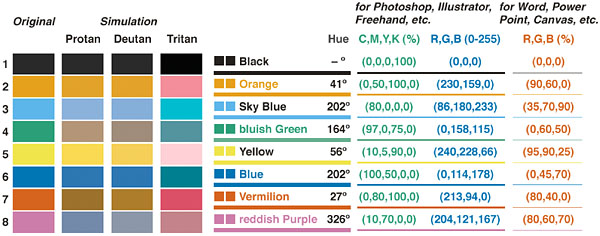
\includegraphics[scale=1.15]{figures/pallete}
 \hspace{1cm}
 \begin{minipage}[b]{0.5\textwidth}
   
\includegraphics[scale=0.55]{figures/ColorBlind_10_discrete}\vspace{10mm}
 \end{minipage}
 \caption{Recommended color palettes for scatter and line plots with several types of data. Credit: Masataka Okabe and Kei Ito (left panel).}
 \label{fig:palettes}
\end{figure*}

\subsubsection{Color recommendations for shading and filled contour plots}

For simple shading, the same advice as for line and scatter plots applies. For more complex cases, e.g.\ parameter constraint plots where pairs of similar colors (for 1$\sigma$ and $2\sigma$ contours) are desired, more care is needed. One collection of color pairs that works reasonably well is illustrated in Figure~\ref{fig:colorcontours} and enumerated as RGB triplets in Table~\ref{tab:colorpairs}. In addition to choosing appropriate color combinations, consider doing the following.
\begin{itemize}
\item Avoid transparency -- it looks fancy, but can easily result in unnecessary color confusion. ``Faux transparency,'' accomplished by using dashed/dotted outlines (as in Figure~\ref{fig:colorcontours}) is often preferable.
\item Place labels directly on or adjacent to (with arrows as needed) shaded areas rather than using a legend (\emph{unlike} Figure~\ref{fig:colorcontours}).
\end{itemize}

\begin{figure*} 
 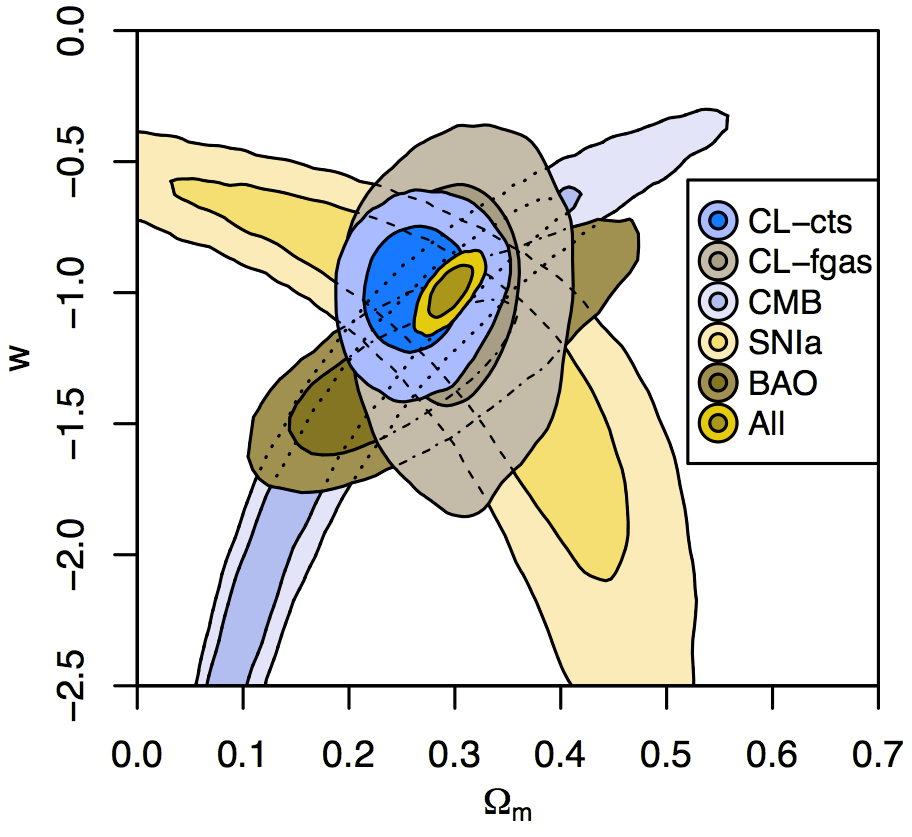
\includegraphics[scale=0.18]{figures/color_contours_deut}
 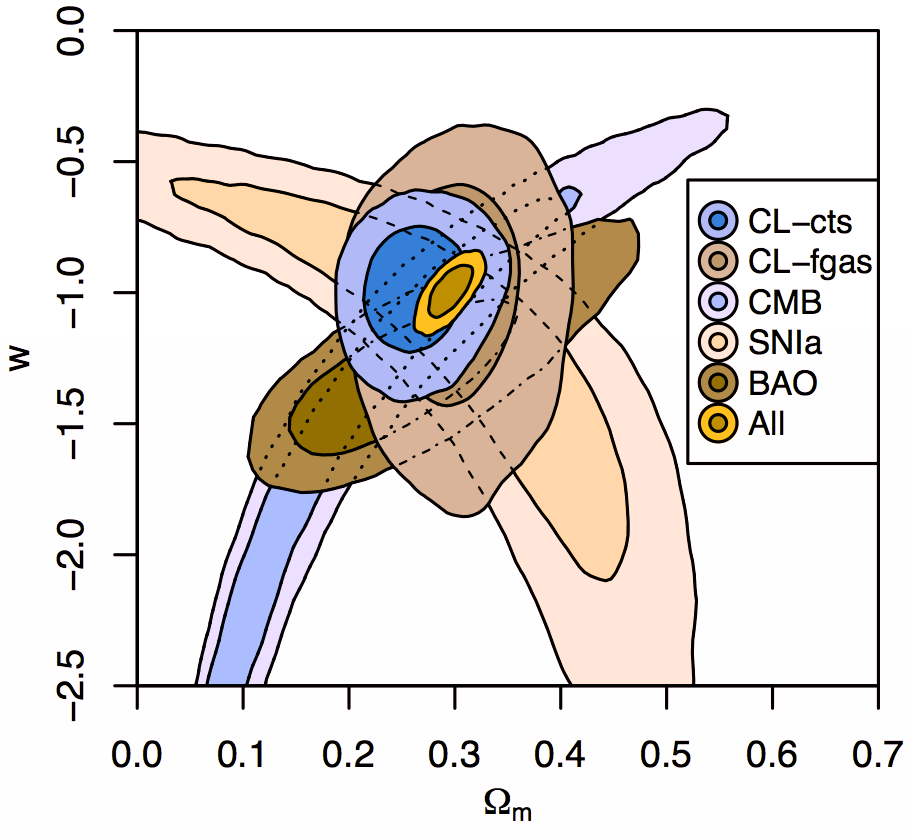
\includegraphics[scale=0.18]{figures/color_contours_prot}
 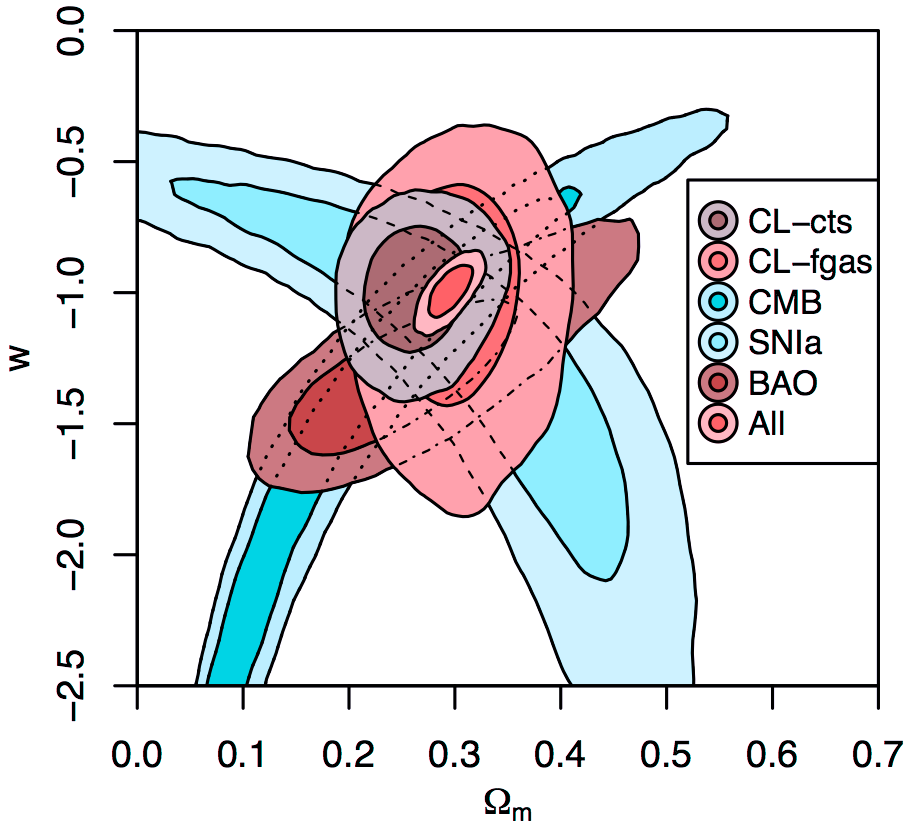
\includegraphics[scale=0.18]{figures/color_contours_trit}
 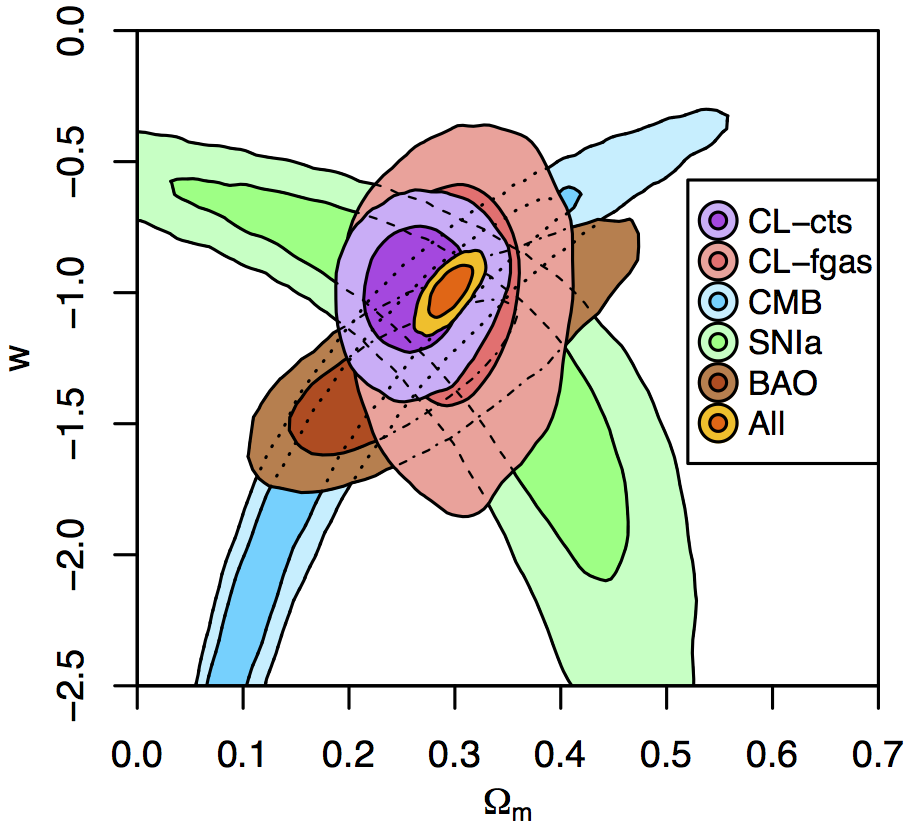
\includegraphics[scale=0.75]{figures/color_contours_normal}
 \hspace{5mm}
 \begin{minipage}[b]{0.6\textwidth}
   \caption{
     Images filtered to simulate the effects of deuteranopia (top-left), protanopia (top-center), and tritanopia (top-right) are compared with the original (bottom-left). This color scheme performs relatively well under the former two (more common) forms of color blindness. (Credit: original by A.~Mantz, distorted versions via \href{http://www.color-blindness.com/coblis-color-blindness-simulator/}{\tt color-blindness.com}.)
   }
   \label{fig:colorcontours}
   \vspace{15mm}
 \end{minipage}
\end{figure*}

\begin{table*}
  \begin{center}
    \caption{
      RGB triplets on the range $[0,1]$, corresponding to the colors used in Figure~\ref{fig:colorcontours}.
    }
    \label{tab:colorpairs}
    \vspace{-1ex}
    \begin{tabular}{lcc}
      \hline
      Color & Dark variant & Light variant \\
      \hline
      Blue & (0.026, 0.818, 1.000) & (0.714, 0.936, 1.000) \\
      Brown & (0.784, 0.294, 0.098) & (0.784, 0.502, 0.294) \\
      Gold & (1.000, 0.400, 0.000) & (1.000, 0.753, 0.000) \\
      Green & (0.333, 1.000, 0.492) & (0.670, 1.000, 0.761) \\
      Purple & (0.737, 0.275, 0.890) & (0.831, 0.686, 0.976) \\
      Red & (1.000, 0.443, 0.442) & (1.000, 0.642, 0.610) \\
      \hline
   \end{tabular}
  \end{center}
\end{table*} 


\subsubsection{Color recommendations for continuous color maps} \label{sec:colormaps}

We expect to streamline this section in the future, with the benefit of experience. In the meantime, here are some options:
\begin{itemize}
\item Single-color gradients are, of course, acceptable.
\item The {\tt b} and {\tt rainbow} color maps in DS9 appear to be relatively robust.
\item One- and two-color gradient maps based on the Okabe \& Ito palette (left panel of Figure~\ref{fig:palettes}) can be easily used in Python thanks to the \href{https://github.com/nesanders/colorblind-colormap}{\tt nesanders/colorblind-colormap} project on GitHub. The GitHub page includes example code.
\end{itemize}

%\subsection{General comments on figures}

%Scripts have been developed showing how to drive {\tt Python} (Andrea Zonca),
%{\tt IDL} (Locke Spencer) and {\tt PGPlot} (Tim Pearson, to be posted soon)
%to produce figures satisfying the requirements.  The companion paper in A\&A
%La\TeX\ format ``Paperplots.tex'' and ``Paperplots.pdf'' show examples
%produced by the scripts and how they are incorporated into papers.  The
%scripts themselves are available at 

%\url{http://github.com/zonca/paperplots/}

%\noindent This is a public site for convenience; no \Planck\ data are used in
%the scripts.  If you need help, ask Andrea, Locke, or Tim
%(see \url{http://www.rssd.esa.int/index.php?project=IDIS&page=people}).

%\medskip

%\subsection{From the A\&A Author's Guide}
%
%
%``If lettered parts of a figure (e.g., 1a, 1b, 1c, etc.) are referred to
%in the figure legend, each part of the figure should be labeled with
%the appropriate letter within the image area. Symbols should be
%explained in the caption and not in the figure.
%
%``Figure legends should concisely label and explain figures and parts of
%figures.  The first sentence of each figure legend should be a
%descriptive phrase, omitting the initial article (the, a, an). In
%multipart figures, the legends should distinguish (a), (b), (c), etc.,
%components of the figure.  Note that if parts are identified in the
%legend as (a), (b), (c), particularly for single figures composed of
%multiple panels, these letters should be clearly labeled in the figure
%itself. Otherwise panels should be referred to by position (top right,
%top left, middle, bottom, etc.). All lines (solid, dashed, dot-dashed,
%dash-dotted, etc.)\ and symbols (filled or open circles, squares,
%triangles, crosses, arrows, etc.) should be explained in the
%legend. Graphics should not be used in figure legends.  The scientific
%discussion of the table or figure contents should appear in the main
%body of the article, not in the table title or figure legend.''

%In general, the first part of a caption should be a phrase ending with a period that functions as a title. This means that captions usually will {\it not\/} start with an article (``a'' or ``the'').  However, there may be exceptions, and brevity should be the rule!  


\subsection{Plots}

\begin{enumerate}
\item {\it Format\/}. Whenever feasible figures should be in EPS, PDF, or another vector format
compatible with the La\TeX\ \verb|\includegraphics| command. Vector graphics can be rendered at any zoom level without pixilation, and (usually) require less disk storage. This is not necessarily the case for images or plots with a very large number of points (e.g., 10's of thousands), however; such graphics should be saved in raster rather than vector format (e.g., PNG, JPEG, TIFF) at print-quality resolution.

\item {\it Line widths for axes, tick marks, etc.\/} Line widths in the range 0.5--0.8\,pt 
 work well.  Lines of width 1\,pt are a bit too heavy for
the boundary box of a figure, although heavier lines can be used when
appropriate for important figure elements to make a clear presentation.  
%In some cases thinner lines may be needed in parts of a figure.  Quantization and
%resolution effects vary from printer to printer; what is seen in test prints
%may not be exactly what will be seen in A\&A.

\item {\it Axes\/}. The figure should be enclosed in a frame on all four
sides, labelled with tick marks, numerical values, and axis labels.  Text
labels should not overlap.

%\item {\it Orientation of numerical values on axes\/}. Numerical values should
%be oriented parallel to the axes.  The reason is straightforward.  If the
%numerical values on the vertical axis are perpendicular to the axis, the space
%they take up horizontally depends on the numbers.  The size of the figure box
%must adjust so that the overall width of the figure is 88, 120, or 180\,mm.  
%The figure frame size then depends on the numerical values on the axis.  Figure
%frames that should be exactly the same size will not be.  Individual images in
%composites will vary in size, and be impossible to align.  The solution,
%fortunately, is simple: run the numbers parallel to the axis.

\item {\it Background grid\/}.  If a grid is needed, it should be drawn with
thin lines (0.5pt?) or grey lines, not dashed or dotted lines.

\item {\it Legends\/}.  A legend within the plot identifying colors and
symbols should be included when necessary.  The legend should not obscure data.
\end{enumerate}

%\subsection{Examples of line plots}
%
%Here is a sample figure set in the three sizes used by A\&A: single-column
%width (Fig.~1), 120\,mm width (Fig.~2), and two-column width (Fig.~3).
%{For more examples, and {\tt IDL} and {\tt Python} scripts that generate
%them, see Paperplots.pdf and associated scripts at}
%
%\url{http://github.com/zonca/paperplots/}
%
%\FIXME{AM: side captions are definitely not accepted by all journals.}
%
%\def\fcaption{Comparison of the joint power spectrum estimates from the three 
%CBI mosaics with the measurements from BOOMERANG, DASI, and MAXIMA.  The 
%rectangles indicate the 68\% confidence intervals on band-power; for 
%BOOME\-RANG, the solid rectangles indicate the 68\% confidence interval for 
%the statistical and sample variance errors, while the hatched rectangles show 
%the amount by which a $\pm1\sigma$ error in the beamwidth 
%($12\parcm9 \pm 1\parcm4$) would shift the estimates (all up or all down 
%together). The {\it black curve} is the joint model (see text).}
%
%% Single-column figure 
%\begin{figure}
%  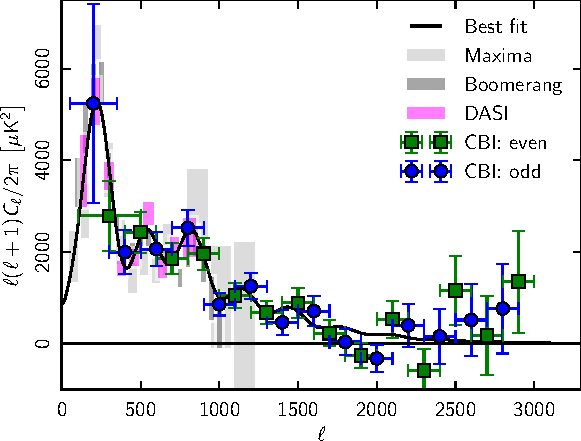
\includegraphics[width=88mm]{Planck_Style_Guide/PlanckFig_lineplot_python_88mm}
%  \caption{\fcaption}
%  \label{fig1col}
%\end{figure}
%
%% Figure with side caption
%\begin{SCfigure}
%  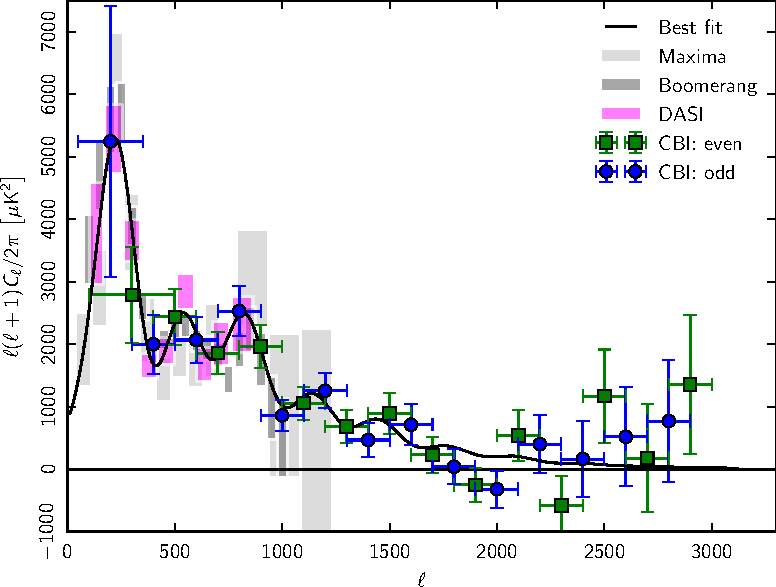
\includegraphics[width=120mm]{Planck_Style_Guide/PlanckFig_lineplot_python_120mm}
%  \caption{120\,mm wide, with caption on the side.\vspace{4cm}}
%  \label{figsidecaption}
%\end{SCfigure}
%
%% Two-column figure
%\begin{figure*} 
%  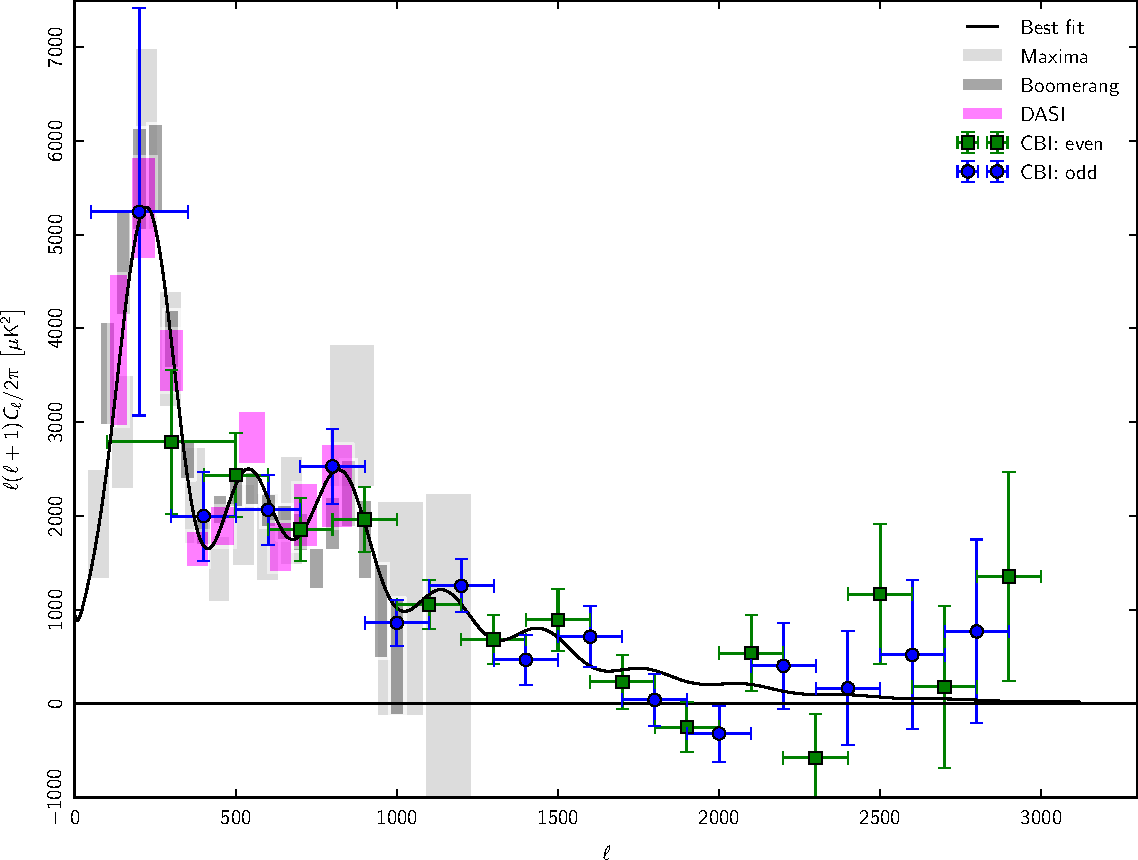
\includegraphics[width=18cm]{Planck_Style_Guide/PlanckFig_lineplot_python_180mm}
%  \caption{\fcaption}
%  \label{fig2col}
%\end{figure*}
%
%The La\TeX\ commands used to produce these are
%\begin{verbatim}
%% Single-column figure 
%\begin{figure}
%  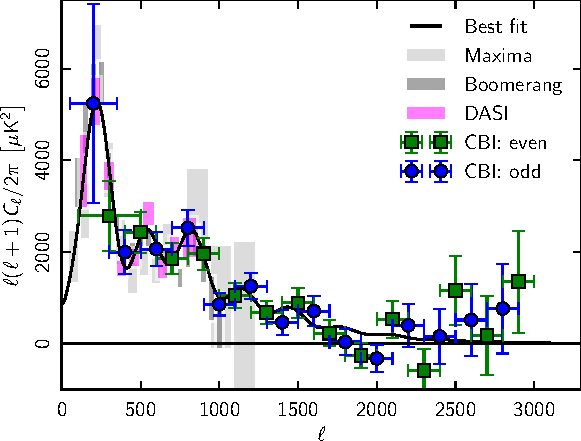
\includegraphics[width=88mm]{Planck_Style_Guide/PlanckFig_lineplot_python_88mm}
%  \caption{\fcaption}
%  \label{fig1col}
%\end{figure}
%
%% Figure with side caption
%\begin{SCfigure}
%  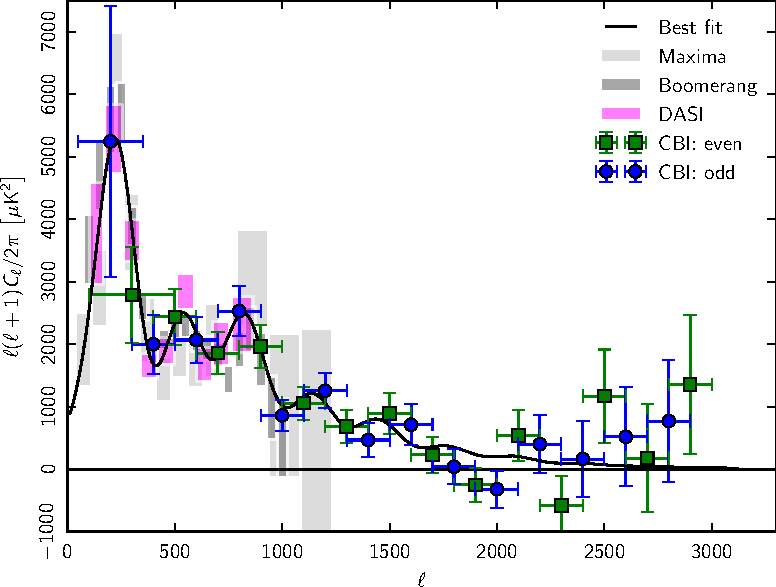
\includegraphics[width=120mm]{Planck_Style_Guide/PlanckFig_lineplot_python_120mm}
%  \caption{120\,mm wide, with caption on the side.\vspace{4cm}}
%  \label{figsidecaption}
%\end{SCfigure}
%
%% Two-column figure
%\begin{figure*} 
%  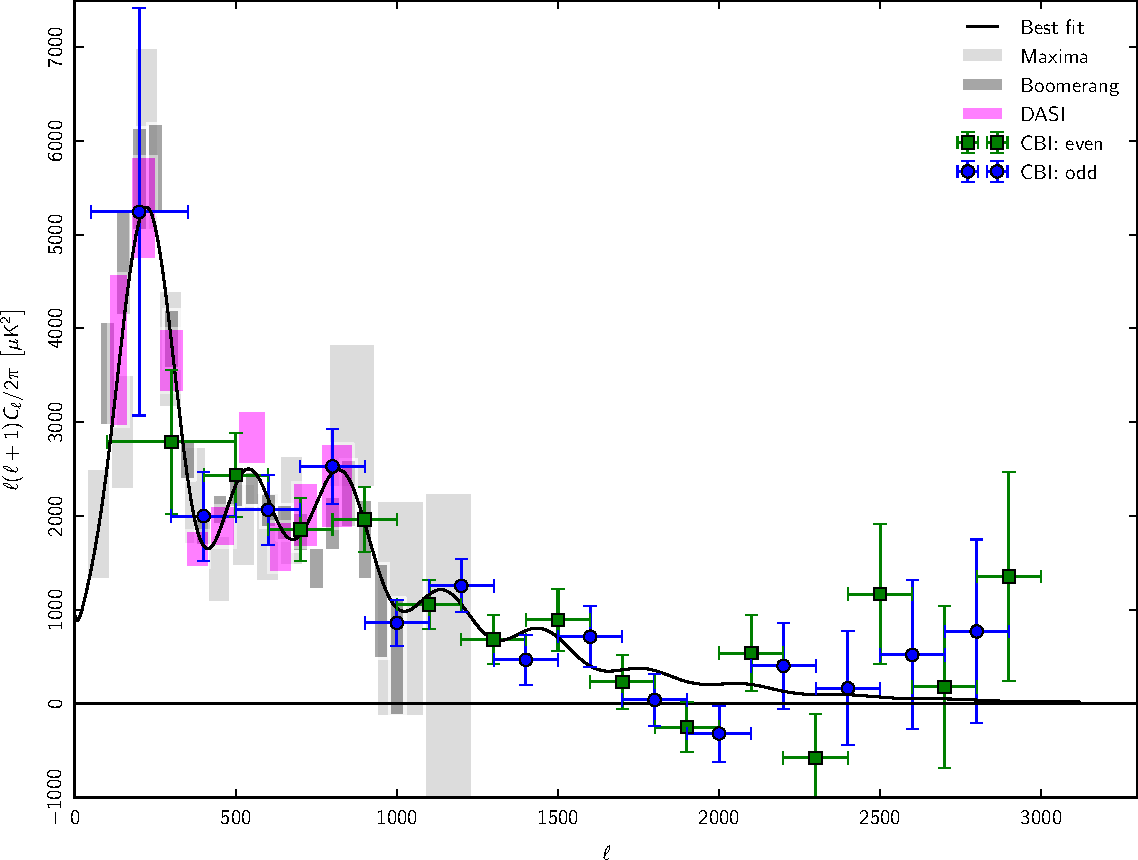
\includegraphics[width=18cm]{Planck_Style_Guide/PlanckFig_lineplot_python_180mm}
%  \caption{\fcaption}
%  \label{fig2col}
%\end{figure*}
%\end{verbatim}
%
\subsection{Images}

Astronomical images are in general ``pseudocolor'' maps, that is, they map
intensity or another quantity onto a color scale chosen to highlight the
features of interest.  

Making a pseudocolor map of a quantity $z$ involves several considerations.

\begin{itemize}
\item
{\it Range}. Choose the minimum and maximum values to
display, $z_1$ and $z_2$ (values outside this range should be replaced by the
minimum or maximum as appropriate, or replaced by an ``undefined'' value).

\item
{\it Transfer function\/}. Apply a linear or nonlinear
transformation to map the range from $z_1$ to $z_2$ to an integer range of
colour indices (often 0 to 255; 256 different color levels is usually
sufficient, although a larger range can be useful in some cases if the
software supports it). One very nonlinear transfer function is ``histogram
equalization;'' while this may be useful for  a first look at a map, it is
only very rarely appropriate for publication.

\item
{\it Color map\/}. Choose color values for each color
index (R, G, B or C, M, Y, K values). Choice of a color map requires careful
deliberation, depending on what features of the map are to be highlighted.
``Undefined'' or unmeasured pixel values should be indicated using a color
that does not appear in the color map (e.g., white or grey).
%\COMMENT{SD: Do we need this?  Or can we make more specific recommendations regarding the color
%map?} 
See Section~\ref{sec:colormaps} for some notes on how to make the map colorblind-friendly.

\end{itemize}
%\smallskip

%One of three standard transfer functions should be used for most map figures.
%\begin{itemize}
%\item The transfer function/color map used in figure~15 of {\it Planck 2013
%results.~I\/}.  This is suitable for maps with low dynamic range and zero mean
%(e.g., the CMB).
%
%\item The transfer function/color map used in figures~9 and 10 of
%{\it Planck 2013 results.~I\/}.  This is suitable for maps with high dynamic
%range and zero mean (e.g., the Planck frequency maps).  It can be used for
%$I$, $Q$, and $U$ maps at all frequencies (but note that different scalings
%are needed for the $I$ maps at 545 and 853\,GHz, which have different units).
%
%\item A one-sided version of the high dynamic range transfer function in the
%previous item, suitable for maps of polarization amplitude $P$ or foregrounds,
%quantities which are inherently positive.  
%\end{itemize}

%\smallskip

%Details of these, with code for use in {\tt IDL} and {\tt Python}, can be found
%in Paperplots.pdf and the code repository (specify).

%If the quantity being mapped is quite different, a completely different colour
%scheme to set it apart may be appropriate.  For example, the ``lensing
%potential map of the Universe'' in the 2013 mission paper (Planck 2013 results.
%I.), figure~18.  These should be discussed with the EB as early as possible to
%ensure consistency between papers.  As far as possible, similar maps should be
%displayed using the same pseudocolour display across all papers. 

%\smallskip\noindent {\it Projection\/}.  Full-sky maps should normally be
%displayed in Mollweide projection in Galactic coordinates.  Sky-patch maps
%should usually be displayed in the orthographic (tan) projection.  When several
%patches are displayed together, they should be on the same scale (mm per
%degree) even if they cover different areas.  Maps from different sources
%intended for direct comparison should always have the same sky coverage, scale,
%and projection; this is best achieved by plotting them with the same graphics
%program.
%
%\smallskip\noindent {\it Resolution\/}.
%Rendering a map for display on screen or paper involves repixelization.
%Typically the printer will use no more than 300 pixels per inch.  Beware of
%information loss in this process.  If the original {\tt HEALPix} pixels are
%smaller than the print pixels, it is advisable to smooth the map before
%rendering.  The visual effect of even mild smoothing can be dramatic.
%Any smoothing should be noted in the caption.
%
%\smallskip\noindent {\it Annotation\/}.  Annotation should be added to the map
%image using a vector-based graphics program, preferably in a separate layer.
%All maps need proper annotation, including colour scale (always) and scale and
%location (except for the standard Mollweide all-sky view in Galactic
%coordinates centred on the Galactic centre).  It should be possible to read
%off the sky location and pixel value.  The caption for a figure containing a
%map or maps should state clearly the source of the data (including the name of
%the file in the PLA when appropriate), the projection, and the coordinate
%system.  For large-area maps in which the lines of longitude and latitude are
%strongly curved, a coordinate grid should be superimposed in the map.  For
%small areas, it may be sufficient to label the coordinates around the edge.
%The colour bar should be labelled in such a way that the value corresponding
%to specific colour can be read off precisely.  In general, and definitely
%for a nonlinear mapping, this requires more than just labelling the end points.
%} 
%
%See Paperplots.pdf and associated scripts at \url{http://github.com/zonca/paperplots/}.
%
%\subsection{Requirements for figures with shading}
%
%See Paperplots.pdf and associated scripts at \url{http://github.com/zonca/paperplots/}.

\subsection{Additional points}

\begin{enumerate}

\item {\it Internal links to figures\/}.  Every internal reference to a figure (or table) should use
\verb|\ref{label}| to ensure that a hyperlink is created in the final PDF file.

\item {\it Sizes and proportions\/}. Pay particular attention to the size of characters and
extraneous white space around figures.  Gauging sizes and proportions is easiest when you produce figures of (or close to) the size they will have in the paper.  Note that for talks, versions of figures with larger fonts and/or symbols may be useful.

\item {\it Captions\/}.  Captions should never start with ``This figure shows \dots''.  Captions should be descriptive enough that the basic content and message of a figure are understandable, independent of the main text.  Conversely, the main text should not excessively duplicate the information in the caption, e.g., about colors and line styles.

\item {\it More on fonts\/}.  Some graphics software packages use outline or
``Hershey'' fonts designed for use with pen-plotters.  They usually include a
sans-serif font that looks similar to Helvetica, but you may need to adjust
the line-thickness as well as the character height to get characters of
appropriate weight.  Typically the line-thickness should be about 1/10 of the
character height. %  \FIXME{to be checked}.

\item {\it Tick marks and numeric labels\/}. Have tick marks projecting out of
the frame only if it is necessary to make them visible.  Use sensible
(rational) tick separations.  Choose units to get numbers without big
exponents.  Avoid overlapping labels.  At least two, and preferably more than
two labels should appear on each axis.  Do not use more significant figures
than are needed in labels (i.e., 10, not 10.00 or 9.999).  It is not necessary
to have the same number of decimal places in axis labels.  For example,
0.01, 0.1, 1, 10, 100 is better than 0.01, 0.10, 1.00, 10.00, 100.00.
Avoid unnecessary trailing zeros.

Sky images should always have coordinates indicated by a labelled frame or
graticule.  Use sexagesimal notation (e.g., h,m,s of RA and d,m,s of Dec) or
decimal degrees, but do not mix the two: if you refer to a source RA of
$12^{\rm h}\,30^{\rm m}$ in the text or a table, do not use 187.5\degree in a
figure!

\item {\it Captions and titles\/}.  Figures have captions.  They {\it should
not\/} have titles or anything else above the frame of the figure.

\item {\it Axis labels\/}. Label axes with the name or description of the
quantity plotted, possibly a symbol, and units if applicable, with the units
in square brackets, e.g., { Detector temperature $T_{\rm det}$ [$\mu$K]},
{ Multipole order $\ell$}, or { Length [mm]}.  However, if logarithms
are involved, { log(length/mm)} is preferable.  { Detector volts [V]}
is incorrect; it should be { Detector reading [V]} or possibly
{ Detector voltage [V]}.  In labels as elsewhere (Sect.~10.8), use exponents,
not fractions in units: { km\,s$^{-1}$}, not { km/s}.  Don't use a dot
to separate units ({ K\,km\,s$^{-1}$}, not { K.km\,s$^{-1}$}).  Don't
invent units for dimensionless quantities (e.g., say { Normalized hit
count}, not { Hit Count [norm.]})  Capitalize labels as normal text (first
letter and proper names only).  Do not use ``{ \#}'' as a synonym for
``number.''

\item {\it Lettering in figures\/}.  Lettering should be in lower-case type,
with the first letter capitalized and no full stop.  Layering type directly
over shaded or textured areas and using reversed type (white lettering on a
coloured background) should be avoided where possible.

%\item {\it Colour\/}.  In general, use colour only if it adds significantly to
%the scientific clarity of the figure.  For example, use colour rather than grey
%and dashed lines if there are many components to be distinguished (more than
%three or four, say).  Always provide a colour bar scale for grey-scale or
%pseudo-colour images.  A graphical legend in the figure, or labelling curves
%individually, is better than describing elements in the caption (avoid ``the
%green dotted line'' etc.; the reader may be viewing a black-and-white copy of
%the paper, or may be colour blind).  

\item {\it Consistency of style and color across figures\/}.  Use a uniform
style for figures throughout the paper.  If a quantity is represented by a red
dashed line in one figure, use the same style for it in other related figures.  

\item{{\it Consistency of style and color for key plots\/}.  In some circumstances, e.g., for plots of cosmology parameter constraints, we will probably want consistent color schemes used across papers.  No specifics are provided here, but the intent will be to follow conventions established in previous DESC papers for the corresponding type of plot. }

\item {\it Multipanel figures\/}.  For a large set of similar figures (e.g.,
SEDs for many objects), use a multipanel figure, which can extend over multiple
pages if necessary.  If there are more than two or three panels, it is usually
best to identify each panel internally (e.g., with the object name) rather
than in the caption.  Avoid phrases like ``middle of third row'' or ``lower
right'' in the text or caption.  Use ``(a),''  ``(b),'' $\dots$ labels if
necessary.  In case two panels are referenced in the caption, use
``{\it Left\/}: \dots,'' ``{\it Right\/}: \dots ,'' ``{\it Upper\/}: \dots,''
``{\it Lower\/}: \dots,''
etc.  To achieve this, type, e.g., \verb|\emph{Left}:| \dots.
Note that the colon is outside the brackets.

\item {\it Mathematical symbols in figures\/}.  Mathematical symbols in
figures should match those in the text. Use \TeX/La\TeX\ to make the symbols
and paste them into the figure if necessary.

\item {\it Geometric distortion\/}.  {\bf Do not} scale the height and width of a figure independently to make it fit a spot in a paper.  The geometrical distortion introduced is unacceptable.  
\end{enumerate}

\section{Tables} \label{sec:tables}

%\subsection{General comments on tables}

%La\TeX\ packages, including A\&A's aa.cls, try to simplify tables by writing
%elaborate overlays for \verb|\halign|, a basic \TeX\ command.    Unfortunately,
%they introduce their own complexity at the same time, as they reduce
%flexibility and make it harder to do many things that are important for the
%readability of tables, things that are simple enough in \verb|\halign|.  Overall,
%it's easier and better to just use \verb|\halign|.  
%
%\verb|\halign| works just fine inside the table environments of aa.cls.  For a
%one-column table, use the \verb|\begin{table}|\dots\verb|\end{table}| environment.  For
%a two-column table, use the
%\verb|\begin{table*}|\dots\verb||\goodbreak\noindent\dots\verb|\end{table*}| environment.
%A template table file is given in \verb|PlanckTable.tex|, which can be found at
%
%\url{http://www.sciops.esa.int/index.php?project=PLANCK&page=Repositories}.
%
%A tutorial on how to use \verb|\halign| to produce tables for Planck is given in
%Sect.~18.2.  Before that, we list some things to do and not to do in tables.

\begin{enumerate}

\item{\it Captions\/}.  Each table should include a caption or equivalent notes that make the content understandable without having to refer to the text.

\item {\it Precision\/}. Excessive numbers of digits should not be given.  In general, the number
of digits used for a quantity should be driven by the uncertainty on that
quantity; in many cases a
single digit on uncertainties is sufficient.  We will follow the specific
policy of the Particle Data Group, described on page~5 of

\url{http://pdg.lbl.gov/2013/reviews/rpp2013-rev-rpp-intro.pdf},

\noindent which says 
\begin{quotation}
\noindent The basic rule states that if the three
highest-order digits of the error lie between 100 and 354, we round to two
significant digits.  If they lie between 355 and 949, we round to one
significant digit.  Finally, if they lie between 950 and 999, we round up to
1000 and keep two significant digits.  In all cases, the central value is given
with a precision that matches that of the error.  So, for example, the result
$0.827\pm0.119$ would appear as $0.83\pm0.12$, while
$0.827\pm0.367$ would turn into $0.8\pm0.4$.
\end{quotation}

There {\it may\/} be cases where using more precision is justified, e.g.,
when there is an important scientific point to make by comparing uncertainties.
However, this should be the exception, and there should be a clear rationale
for using increased numbers of digits.

%\item Footnotes in tables should be identified by roman superscript letters,
%which can be set with \verb|\tablefootmark{}| and \verb|\tablefoottext{}|.  Better yet, make tables with \verb|\halign| as described below starting in Sect.~18.2, and use the prescription given in Sect.~18.15.
%
%\item Don't use check marks in tables as a substitute for ``yes'' or ``Y.''
%It's tacky.  Better still, don't use boolean columns in tables at all.

\item {\it Missing values\/}. Missing values should be indicated by an ellipsis, ``\dots,'' obtained
with the \verb|\ldots| command (or \verb|\nodata| in ApJ articles).  Don't try to produce an ellipsis with periods (full
stops).  The spacing will be wrong...

\item {\it Alignment\/}. When entries in a column are to be compared, align the decimal points in
both the quantity and the uncertainty. Align $\pm$ symbols when possible. \FIXME{Add some pointers/examples of how to do this.}

% \midinsert
% \begingroup
% \ninepoint
% \centerline{\bf Table 2.} 
% \centerline{\csc Decimal Point Alignment}
% \vglue -10pt
% \setbox\tablebox=\vbox{
%    \newdimen\digitwidth 
%    \setbox0=\hbox{\rm 0} 
%    \digitwidth=\wd0 
%    \catcode`*=\active 
%    \def*{\kern\digitwidth}
% %
%    \newdimen\decimalwidth 
%    \setbox0=\hbox{$.0$} 
%    \decimalwidth=\wd0 
%    \catcode`!=\active 
%    \def!{\kern\decimalwidth}
% %
% \halign{\hbox to 1.4in{#\leaderfil}\tabskip=0.75em&
%    \hfil#\hfil\tabskip=0pt\cr
% \noalign{\doubleline}
% \omit&30\,GHz\cr
% \noalign{\vskip 5pt\hrule\vskip 5pt}
% \omit\hfil Example 1\hfil\cr
% \noalign{\vskip 4pt}
% $\Delta T_{30}$ [$\mu$K]          &$38.6\pm13.2$\cr
% $\Delta T_{30}/T$                 &$*1.7\pm*0.7$\cr
% \omit&\cr
% \omit\hfil Example 2\hfil\cr
% \noalign{\vskip 4pt}
% $\Delta T/T$ per pixel            &$(5.9\pm0.6)\times10^{-3}$\cr
% $N_{\rm feeds}$                   &$1.2\pm0.2$\cr
% \noalign{\vskip 5pt\hrule\vskip 3pt}}}
% \endPlancktable

% \endgroup
% \endinsert

%\item Tables should have a double rule at the top, a single rule between
%headings and the body of the table, and a rule at the bottom.  See Sect.~18.9.
%
%\item The spacing of lines in tables often requires no special attention, at
%least when there is no complicated structure.  However, one case that occurs
%fairly frequently in Planck papers and requires special attention is that of
%table values with asymmetrical errors (Table~3).  Extra space in needed and
%easily obtained in this example with \verb|\noalign{\vskip 4 pt}| between the lines
%(see Sect.~18.7).

% \midinsert
% \begingroup
% \ninepoint
% \centerline{\bf Table 3.} 
% \centerline{\csc Spacing With Asymmetric Errors}
% \vglue -25pt
% \setbox\tablebox=\vbox{
%    \newdimen\digitwidth 
%    \setbox0=\hbox{\rm 0} 
%    \digitwidth=\wd0 
%    \catcode`*=\active 
%    \def*{\kern\digitwidth}
% %
%    \newdimen\signwidth 
%    \setbox0=\hbox{+} 
%    \signwidth=\wd0 
%    \catcode`!=\active 
%    \def!{\kern\signwidth}
% %
% \halign{\hbox to 1in{#\leaderfil}\tabskip=1.0em&\hfil#\hfil&\hfil#\hfil&\hfil#\hfil&\hfil#\hfil&\hfil#\hfil&\hfil#\hfil&\hfil#\hfil&\hfil#\hfil\tabskip=0pt\cr 
% \noalign{\vskip 5pt}
% \noalign{\doubleline}
% \omit& $r_{x}$\cr
% \omit\hfil Sector\hfil &[Mpc]& $D_n$& $M_n$& $D_T$& $M_T$& $D_n\times D_T$& $M_{nT}$& $M_{\rm SZ}$\cr 
% \noalign{\vskip 3pt\hrule\vskip 5pt}
% \multispan9\hfil{\bf Bad}\hfil\cr
% \noalign{\vskip 5pt}
% West     &$1.173^{+0.0003}_{-0.003}$ & $2.00^{+0.03}_{-0.03}$ & $1.73^{+0.03}_{-0.03}$ &$3.0^{+0.7}_{-0.6}$  & $2.6^{+0.4}_{-0.4}$  & $6.0^{+1.4}_{-1.1}$&$2.3^{+0.2}_{-0.2}$&$1.95^{+0.45}_{-0.02}$\cr
% Southeast&$0.9778^{+0.0002}_{-0}$    & $2.43^{+0.02}_{-0.02}$ & $2.10^{+0.01}_{-0.01}$ &$1.3^{+1.8}_{-0.6}$ & $1.3^{+1.3}_{-1.3}$  & $3.1^{+1.6}_{-1.1}$&$1.6^{+0.3}_{-0.1}$&$2.03^{+0.14}_{-0.04}$\cr
% \noalign{\vskip 5mm}
% \multispan9\hfil {\bf Good}\hfil\cr
% \noalign{\vskip 5pt}
% West     &$1.173^{+0.0003}_{-0.003}$ & $2.00^{+0.03}_{-0.03}$ & $1.73^{+0.03}_{-0.03}$ &$3.0^{+0.7}_{-0.6}$  & $2.6^{+0.4}_{-0.4}$  & $6.0^{+1.4}_{-1.1}$&$2.3^{+0.2}_{-0.2}$&$1.95^{+0.45}_{-0.02}$\cr
% \noalign{\vskip 4pt}
% Southeast&$0.9778^{+0.0002}_{-0}$    & $2.43^{+0.02}_{-0.02}$ & $2.10^{+0.01}_{-0.01}$ &$1.3^{+1.8}_{-0.6}$ & $1.3^{+1.3}_{-1.3}$  & $3.1^{+1.6}_{-1.1}$&$1.6^{+0.3}_{-0.1}$&$2.03^{+0.14}_{-0.04}$\cr
% \noalign{\vskip 5pt\hrule\vskip 3pt}}}
% %\endPlancktable                    % ends one-column \halign
% \endPlancktable                 % ends two-column \halign
% \endgroup

% \endinsert

%\item Blank spaces in the input La\TeX\ file are often ignored, and adding
%spaces in table input files can improve the human readability of a table.  But
%there is one case in tables to watch out for.   In \verb|\halign|, spaces following
%ampersands before a table entry are ignored; however, {\it spaces between a
%table entry and the next ampersand are {\bf not} ignored}, and change the
%spacing of column entries.  Consider the following lines, used in Table~4.  
%
%\verb|Quantity&15&4&10&8\cr|
%
%\verb|Quantity& 15& 4& 10& 8\cr|
%
%\verb|Quantity& 15 & 4 & 10 & 8 \cr|
%
%\medskip

% \midinsert
% \begingroup
% \ninepoint
% \centerline{\bf Table 4.} 
% \centerline{\csc Some Blanks Matter}
% \vglue -10pt
% \setbox\tablebox=\vbox{
%    \newdimen\digitwidth 
%    \setbox0=\hbox{\rm 0} 
%    \digitwidth=\wd0 
%    \catcode`*=\active 
%    \def*{\kern\digitwidth}
% %
%    \newdimen\decimalwidth 
%    \setbox0=\hbox{$.0$} 
%    \decimalwidth=\wd0 
%    \catcode`!=\active 
%    \def!{\kern\decimalwidth}
% %
% \halign{\hbox to 1.0in{#\leaderfil}\tabskip=0.75em&
%    \hfil#\hfil&
%    \hfil#\hfil&
%    \hfil#\hfil&
%    \hfil#\hfil\tabskip=0pt\cr
% \noalign{\doubleline}
% Quantity&15&4&10&8\cr
% Quantity& 15& 4& 10& 8\cr
% Quantity& 15 & 4 & 10 & 8 \cr
% \noalign{\vskip 5pt\hrule\vskip 3pt}}}
% \endPlancktable

% \endgroup
% \endinsert

%\noindent The first two lines produce identical output, but the
%third line produces different output.  Given the importance of precise
%alignment of column entries (as discussed above in Table~2), the rule is
%{\bf no spaces before ``\verb|&|''s and ``\verb|\cr|''s}.

\end{enumerate}

%\noindent{\bf The remainder of this section has not been copied, as it is even more technical and specific to the \verb|\halign| method of formatting tables.}







%\bibliographystyle{bib/refs}
%\bibliography{bib/references}

\end{document}
